\documentclass[12pt]{article}
\usepackage[utf8]{inputenc}
\usepackage[a4paper, margin=1in]{geometry}
\usepackage{graphicx}
\usepackage{subcaption}
\usepackage{hyperref}
\usepackage{booktabs}
\usepackage{titlesec}
\usepackage{enumitem}
\usepackage{xcolor}
\usepackage{caption}
\graphicspath{{figures/}}
\definecolor{UdGblue}{RGB}{0, 51, 153}
\titleformat{\section}{\large\bfseries}{\thesection}{1em}{}
\titleformat{\subsection}{\normalsize\bfseries}{\thesubsection}{1em}{}
\usepackage{fancyhdr}
\pagestyle{fancy}
\fancyhf{}
\renewcommand{\headrulewidth}{0.4pt} 
\usepackage{pgfgantt}
\usepackage{float}
\usepackage{booktabs}
\usepackage{pgfgantt}
\usepackage{float}
\setlength{\headheight}{15pt}
\usepackage{array}
\usepackage[table]{xcolor}
\usepackage{graphicx}
\usepackage{float}
\usepackage{url}
\usepackage{hyperref}
\usepackage{doi}
\usepackage{amsmath}
\usepackage{amssymb}

\lhead{Robust View-Invariant Feature Matching for Side-Scan Sonar Imagery}


\rhead{Page \thepage}
\patchcmd{\chapter}{\thispagestyle{plain}}{\thispagestyle{fancy}}{}{}

\begin{document}

% --- TITLE PAGE ---
\begin{titlepage}
    \centering
    {\Large \textbf{Universitat de Girona}} \\
    \vspace{0.2cm}
    \textbf{Master in Intelligent Robotic Systems (MIRS)} \\
    \vspace{0.5cm} 
    

    \begin{center}
        
\includegraphics[height=3.0cm]{assets/udg_logo.png}
    \end{center}
    
    \vspace{0.5cm}
    \textbf{Master Thesis (3501MO3382/2026)} \\
    \vspace{1.5cm}
    
    \hrule
    \vspace{0.5cm}
    {\huge \textbf{Beyond SIFT: Robust View-Invariant Feature Matching for Side-Scan Sonar Imagery}} \\
    \vspace{0.5cm}
    \hrule
    
    \vspace{2cm}

    \begin{center}
        \begin{minipage}[t]{0.35\textwidth}
            \centering
            \textbf{Student Name}\\
            Taqi Hamoda
        \end{minipage}
        \hspace{0.01cm} 
        \begin{minipage}[t]{0.35\textwidth}
            \centering
            \textbf{Student ID}\\
            U1999412
        \end{minipage}
    \end{center}

    \vspace{1.0cm} 

    % --- MAIN SUPERVISOR ---
    \textbf{Main Supervisor Name}\\
    Nuno Gracias
    \vfill 

    \textbf{Submission date:} June 8, 2026

\end{titlepage}
\newpage
\tableofcontents
\newpage

\begin{abstract}
Side-scan sonar (SSS) is essential for large-scale underwater mapping and autonomous navigation, yet its acoustic acquisition process introduces severe view-dependent distortions, non-linear intensity variations, and speckle noise. These artifacts degrade the performance of traditional local feature detectors, like SIFT, when establishing cross-view correspondences. To address this, we present a novel, physics-informed self-supervised learning framework based on the DINOv3 architecture. Designed for the strict computational constraints of Autonomous Underwater Vehicles (AUVs), our framework utilizes an efficient ConvNeXt-tiny backbone. We introduce a Lambertian acoustic reflection model that decouples intrinsic seabed reflectivity from view-dependent artifacts such as acoustic shadows and path loss. Furthermore, we employ domain-adaptive techniques to stabilize high-resolution dense feature extraction without manual annotations. Evaluations demonstrate that our methodology extracts robust, view-invariant semantic representations that significantly improve cross-view correspondence reliability, ultimately enhancing the deployment autonomy of underwater robotic platforms.
\end{abstract}

\section{Introduction}

\begin{figure}[h]
\centering
\includegraphics[width=\textwidth]{assets/sss.png}
\caption{Side-Scan Sonar deployment on a towfish connected to a survey vessel. Figure adapted from \cite{sss_book}.}
\label{fig:sss_towfish}
\end{figure}

Underwater robotic perception is severely constrained by the marine environment. Due to absorption and scattering, electromagnetic radiation attenuates rapidly in water, limiting high-resolution optical sensors to ranges under 10~m~\cite{can2025_sss,katrusha2025}. Conversely, acoustic energy propagates with low attenuation, enabling sound waves to travel hundreds of meters even in turbid or low-light conditions. As such, Side-Scan Sonar (SSS) has become the primary modality for large-scale seafloor mapping, long-range target detection, and autonomous navigation~\cite{antoni2016,hayat2025}.

Unlike optical cameras, SSS image formation is governed by acoustic acquisition dynamics~\cite{antoni2016, can2025_physdnet}. As illustrated in Figure~\ref{fig:sss_towfish}, laterally mounted transducers on a moving platform emit fan-shaped pulses perpendicular to the trajectory. The returning echoes are recorded over time and converted to range assuming a constant sound speed of $1500\,\mathrm{m/s}$, yielding a continuous 2D backscatter intensity map~\cite{antoni2016,hayat2025}. Traditionally, this process is approximated via a Lambertian model:
\begin{equation}
I(x,y) = \rho(x,y) \cdot \cos(\theta(x,y)) \cdot L(x,y),
\end{equation}
where the recorded intensity $I(x,y)$ is a function of the intrinsic seabed reflectivity $\rho(x,y)$, the local incidence angle $\theta(x,y)$, and the acoustic propagation loss $L(x,y)$~\cite{can2025_physdnet,antoni2016}.

However, this simplified model fails to capture true acoustic complexities. Real SSS transducers emit non-uniform power profiles that diminish at the beam edges and vary across side lobes~\cite{yvan_petillot}. Furthermore, topographic occlusions create acoustic shadows, and multiplicative speckle noise inherently corrupts the signal~\cite{katrusha2025,alan2022}. The resulting imagery is highly viewpoint-dependent; different survey directions yield drastically altered intensity patterns and shadow geometries for identical seafloor structures.

These severe physical artifacts severely bottleneck automated perception. Viewpoint dependencies and non-uniform intensities result in poor repeatability for traditional handcrafted keypoint extractors (e.g., SIFT, SURF), causing high matching errors and rendering real-time analytical interpretation unreliable~\cite{can2025_sss,katrusha2025,fu2025,hayat2025}. To overcome these limitations, recent research has turned toward deep Self-Supervised Learning (SSL). By leveraging large-scale, unlabeled sonar data, SSL frameworks enable the extraction of physically invariant features without relying on scarce manual annotations~\cite{oriane2025,alan2022}, offering a promising pathway for robust autonomous underwater navigation.

\begin{figure}[h]
\centering
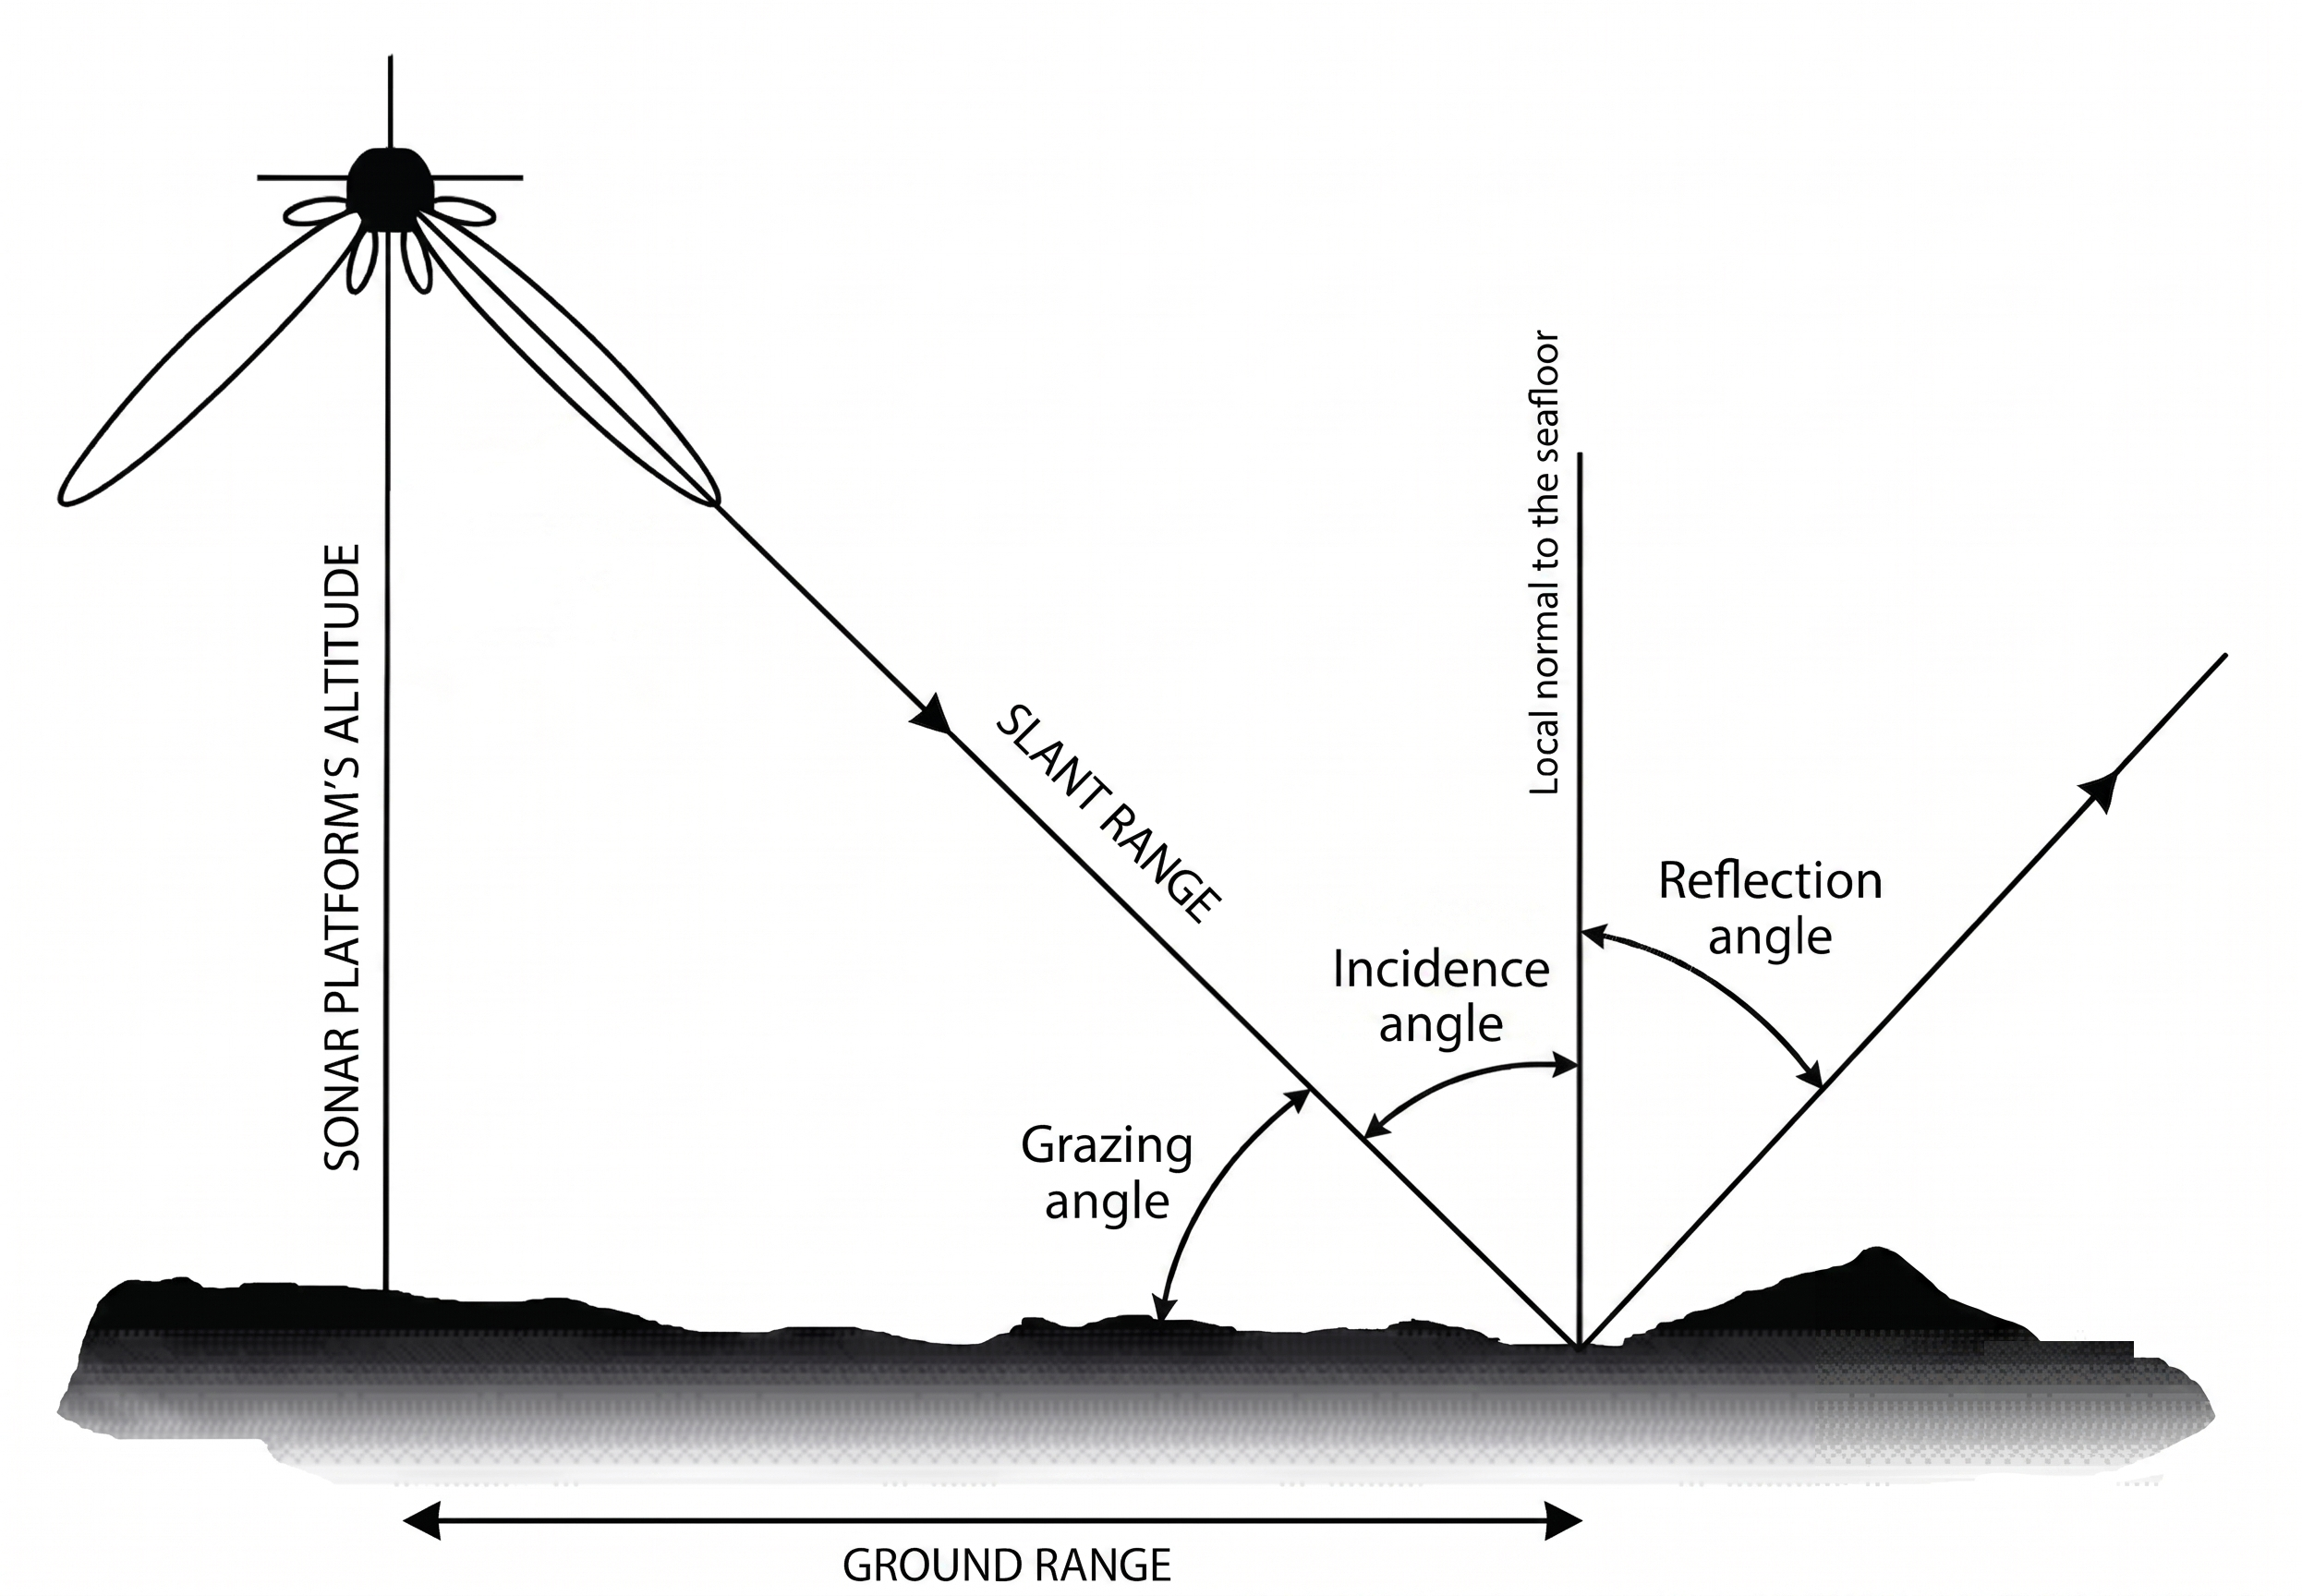
\includegraphics[width=\textwidth]{assets/lambertian.png}
\caption{The Lambertian physics model for the SSS modality. Figure adapted from \cite{sss_handbook}}
\label{fig:lambertian}
\end{figure}

\subsection{State of the Art in Feature Extraction and Matching}

\begin{figure}[htbp]
  \centering
  \begin{subfigure}[b]{0.48\linewidth}
    \centering
    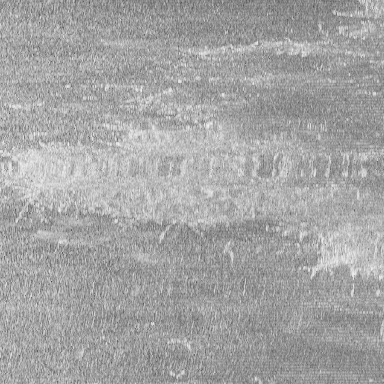
\includegraphics[width=\linewidth]{assets/distortion.png}    
  \end{subfigure}
  \hfill
  \begin{subfigure}[b]{0.48\linewidth}
    \centering
    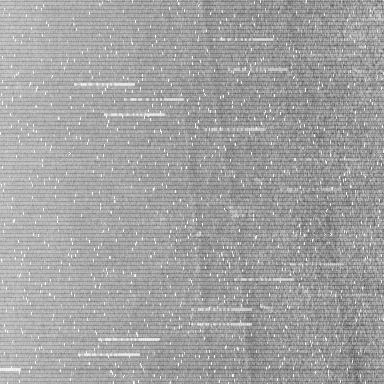
\includegraphics[width=\linewidth]{assets/speckle_noise.png}
  \end{subfigure}
  \caption{Acoustic degradation in SSS imagery: rotation distortion and view-dependence (left); severe speckle noise and acoustic stripe artifacts (right).}
  \label{fig:sss_challenges}
\end{figure}

Correspondence matching in SSS imagery is hindered by the geometric distortions and extreme speckle noise~\cite{can2025_sss,katrusha2025}. Handcrafted descriptors (e.g., SIFT, SURF, AKAZE) rely on local intensity gradients, which are disrupted by acoustic artifacts and view-dependent backscatter, leading to poor repeatability in underwater domains~\cite{lowe2004,can2025_sss,fu2025}. 

As such, recent approaches employ deep learned detectors (e.g., SuperPoint, DISK) and Transformer-based matchers (e.g., LightGlue, LoFTR)~\cite{katrusha2025,fu2025}. LightGlue uses iterative self- and cross-attention with adaptive computation for efficient sparse matching. Conversely, LoFTR bypasses detection entirely, utilizing a coarse-to-fine Transformer architecture to establish dense matching across texture-poor or low-contrast regions~\cite{katrusha2025,fu2025}.

Despite success in optical domains, acoustic benchmarks by Katrusha et al.~\cite{katrusha2025} reveal severe performance degradation under wave distortion and stripe noise, exposing critical architectural trade-offs:
\begin{itemize}
    \item \textbf{Sparse Methods (SuperPoint + LightGlue):} Maintain relative accuracy under noise but yield sparse correspondences, failing to provide the dense alignment needed for precise mapping or change detection.
    \item \textbf{Dense Methods (LoFTR):} Achieve high spatial coverage (up to 97\%) but are sensitive to low-contrast artifacts, resulting in a low inlier rate ($\sim$8\%), high reprojection errors, and an prohibitive computational footprint (up to 15$\times$ more resource-intensive) for real-time AUV deployment.
\end{itemize}

A foundational limitation is that these networks are typically deployed "out-of-the-box" using pre-trained optical weights~\cite{katrusha2025}. Without domain-specific fine-tuning, they fail to generalize to acoustic physics, relying instead on 2D homographic approximations that disregard 3D seafloor topography.

This domain gap worsens in cross-modal alignment (e.g., pairing SSS with optical imagery). To enforce structural consistency across differing sensor physics, symmetric epipolar distance is introduced to constrain the geometry:
\begin{equation}
d(p_1,p_2) = \frac{(p_2^\top F p_1)^2}{\|F p_1\|^2} + \frac{(p_1^\top F^\top p_2)^2}{\|F^\top p_2\|^2},
\end{equation}
where $F \in \mathbb{R}^{3 \times 3}$ is the fundamental matrix mapping corresponding points~\cite{fu2025}. However, optimizing this constraint requires features invariant to the modalities physics, which optical models cannot provide.

To bridge this gap, this work introduces self-supervised training and fine-tuning of DINOv3 directly on large-scale SSS datasets. By embedding acoustic image formation constraints into the architecture, we learn robust, modality-invariant representations. This addresses the dual challenge of underwater perception: enabling dense, noise-resilient correspondences for same-modality SSS matching, while providing the high-level semantic abstractions necessary for robust opti-acoustic cross-modal alignment.

\subsection{Contributions}
To address acoustic degradation, viewpoint dependency, and domain gaps in underwater perception, this thesis introduces a physics-informed, self-supervised learning framework for SSS imagery. The primary contributions are:

\begin{itemize}
    \item \textbf{Lightweight Self-Supervised Foundation Model:} We adapt the DINOv3 framework with an efficient ConvNeXt-Tiny backbone. This architecture generates robust, zero-shot semantic features while satisfying the strict computational and payload constraints of autonomous underwater vehicles (AUVs).
    
    \item \textbf{Physics-Informed Feature Learning:} By embedding a Lambertian acoustic reflection model into the self-supervised pipeline, the framework decouples intrinsic seafloor reflectivity from viewpoint-dependent artifacts, including acoustic shadows, beam patterns, and slant-range propagation loss.
        
    \item \textbf{Geometric Opti-Acoustic Co-Registration Framework:} We develop a cross-modal alignment framework that uses reconstructed 3D optical geometry for multi-modal matching. This physics-based approach achieves pixel-level registration accuracy and provides an automated, scalable pipeline to generate co-registered opti-acoustic datasets for downstream learning.
\end{itemize}

\section{Backbone Architecture: ConvNeXt}

\begin{figure}[h]
\centering
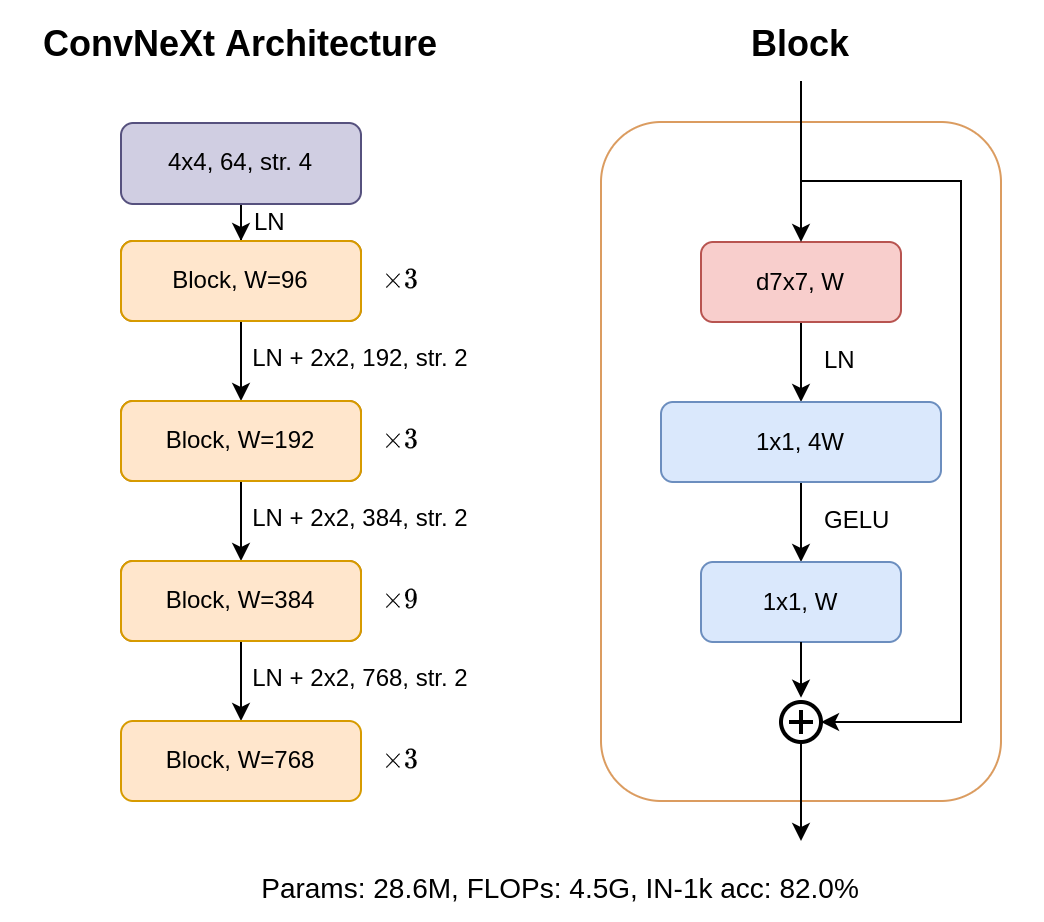
\includegraphics[width=\textwidth]{assets/convnext.png}
\caption{The ConvNeXt-Tiny architecture used in the backbone.}
\label{fig:convnext}
\end{figure}

Autonomous underwater perception via Side-Scan Sonar (SSS) requires handling severe geometric distortions and non-linear intensity variations \cite{can2025_sss, katrusha2025}. While Vision Transformers (ViTs) yield strong performance, their quadratic computational complexity restricts deployment on resource-constrained AUVs \cite{liu2022, oriane2025}. Therefore, we adopt ConvNeXt-tiny as the feature extractor within the DINOv3 self-supervised framework \cite{liu2022, oriane2025}. ConvNeXt modernizes the ResNet design space by preserving convolutional inductive biases—such as translation equivariance and local connectivity—while integrating hierarchical Transformer advantages \cite{liu2022}.

\subsection{Modernizing ResNet}

ConvNeXt updates the baseline ResNet-50 via an improved training recipe (AdamW, 300 epochs, Mixup, CutMix, RandAugment), raising ImageNet top-1 accuracy from 76.1\% to 78.8\% \cite{liu2022}. Structural enhancements span five categories: macro design, ResNeXt-style cardinality, inverted bottlenecks, large kernels, and micro refinements. Crucially, ConvNeXt's convolutional locality aligns with the ping-by-ping, locally correlated nature of SSS data, optimizing sediment texture and object boundary detection \cite{antoni2016, can2025_physdnet}.

\subsection{Key Design Choices}

\paragraph{Macro design}
ConvNeXt-tiny adopts the Swin-T stage compute ratio (3, 3, 9, 3 blocks) and replaces the ResNet 7×7 stride-2 stem and max-pool with a 4×4 stride-4 "patchify" stem to mirror ViT patch embedding \cite{liu2022}.

\paragraph{Depthwise conv + inverted bottleneck}
Depthwise 7×7 convolutions are placed before the 1×1 layers to separate spatial and channel mixing. An inverted bottleneck expands the MLP hidden dimension to $C_\text{hidden} = 4 \cdot C_\text{input}$, concentrating expensive operations in fewer channels \cite{liu2022}.

\paragraph{Large kernels}
The 7×7 depthwise kernel expands the receptive field to match Swin Transformer window sizes, allowing the model to capture large-scale topographic features and acoustic shadows in SSS imagery \cite{liu2022, can2025_sss}.

\paragraph{Micro refinements}
- Replaces ReLU with GELU.
- Minimizes activations and normalizations (one GELU and one LayerNorm per block).
- Substitutes BatchNorm with LayerNorm to improve training stability \cite{liu2022}.

\subsection{ConvNeXt V2: Co-designing with Masked Autoencoders}

While ConvNeXt V1 scales efficiently under supervised learning, applying mask-based self-supervised learning—such as Masked Autoencoders (MAE)—induces "feature collapse" \cite{ConvNextV2}. Training directly on masked inputs causes the dimension-expansion MLP layers to yield dead or saturated feature maps, resulting in redundant channel activations and degraded feature diversity \cite{ConvNextV2}.

To mitigate this, ConvNeXt V2 introduces Global Response Normalization (GRN) directly after the MLP expansion layer, rendering the original LayerScale operation redundant \cite{ConvNextV2}. GRN enhances inter-channel competition by aggregating spatial features into a channel-wise L2-norm vector, applying divisive normalization to establish mutual inhibition, and calibrating the original input responses \cite{ConvNextV2}. This architecture maintains feature diversity without significant parameter or computational overhead.

Furthermore, co-designing ConvNeXt V2 with a Fully Convolutional Masked AutoEncoder (FCMAE) pre-training framework treats the masked image as a 2D sparse array. Utilizing sparse convolutions to process only visible patches prevents the network from copying information from masked regions, substantially boosting pre-training efficiency \cite{ConvNextV2}.

\subsection{Computational Efficiency}

ConvNeXt-tiny achieves 82.1\% ImageNet top-1 accuracy at 4.5 GFLOPs, outperforming Swin-T (81.3\%) at equivalent compute, while delivering up to 49\% higher inference throughput on A100 GPUs (TF32, channels-last) \cite{liu2022}. Integrated into DINOv3, ConvNeXt-tiny enables efficient high-resolution feature extraction on edge devices, accommodates low-bitwidth quantization better than Transformers, and generates sharp, semantically consistent dense features across diverse sonar resolutions \cite{oriane2025, hayat2025, fu2025}.

\section{Self-Supervised Learning with DINOv3}

\begin{figure}[h]
\centering
\includegraphics[width=\textwidth]{assets/dino.png}
\caption{The Student-Teacher training paradigm employed by DINO.}
\label{fig:dino}
\end{figure}

Visual representation learning has shifted from supervised to self-supervised methods that exploit unlabelled data \cite{asifullah2025}. This is particularly important for SSS imaging, where data acquisition and expert annotation are expensive and time-consuming \cite{hayat2025, alan2022}.

DINOv3 employs a self-distillation framework combining global discriminative alignment, local masked reconstruction, feature regularization, and Gram anchoring to learn robust representations for SSS data.

\subsection{Self-Distillation Framework}

DINOv3 uses a teacher-student architecture where the teacher is an exponential moving average (EMA) of the student weights \cite{oriane2025, asifullah2025}. The student matches the teacher's output distributions instead of using contrastive pairs.

The pre-training loss is:
\begin{equation}
\mathcal{L}_{\text{Pre}} = \mathcal{L}_{\text{DINO}} + \mathcal{L}_{\text{iBOT}} + 0.5 \cdot \mathcal{L}_{\text{Gram}} + 0.1 \cdot \mathcal{L}_{\text{DKoLeo}}
\end{equation}

A final layer normalization is applied to backbone outputs of both global and local crops to stabilize dense feature learning late in training \cite{oriane2025}.

\subsubsection{Global Discriminative Loss ($\mathcal{L}_{\text{DINO}}$)}

The DINO objective enforces view-invariance at the image level using a multi-crop strategy: the student sees two global crops and several local crops, while the teacher sees only global crops \cite{oquab2024, oriane2025}.

Output distributions are obtained via a projection head + softmax over $K$ dimensions. To avoid collapse, DINOv3 uses Sinkhorn-Knopp centering instead of the original centering-sharpening \cite{caron2021, oquab2024}. The loss aligns the student distribution $P_s$ with the centered teacher distribution $P_t$:

\begin{equation}
\mathcal{L}_{\text{DINO}} = -\sum_{v \in V} \sum_{v' \in V_{\text{global}}} P_t(x_{v'}) \log P_s(x_v)
\end{equation}

This promotes features invariant to geometric distortions and speckle noise typical in SSS imagery \cite{hayat2025}.

\subsubsection{Masked Latent Reconstruction ($\mathcal{L}_{\text{iBOT}}$)}

The iBOT objective adds dense prediction capability by reconstructing masked patch tokens using the teacher's unmasked representations \cite{oquab2024, oriane2025}:

\begin{equation}
\mathcal{L}_{\text{iBOT}} = -\sum_{i \in \mathcal{M}} P_{t_i}^{\text{patch}} \log P_{s_i}^{\text{patch}}
\end{equation}

Sinkhorn-Knopp centering is also applied to patch projections. This helps the model infer missing sonar information from acoustic shadows and seabed textures, improving local feature quality on datasets such as BenthiCat \cite{hayat2025, oriane2025}.

\subsubsection{Feature Regularization ($\mathcal{L}_{\text{DKoLeo}}$)}

KoLeo regularization prevents feature collapse by encouraging uniform hyperspherical distribution within each batch \cite{oquab2024, oriane2025}:

\begin{equation}
\mathcal{L}_{\text{KoLeo}} = -\frac{1}{n} \sum_{i=1}^{n} \ln \left( \min_{j \neq i} \| z_i - z_j \| \right)
\end{equation}

This maximizes minimum distances between samples, improving class separability in downstream benthic tasks.

\subsection{Gram Anchoring}

Long training schedules and high resolutions often degrade dense feature maps, causing patch-level inconsistency and noisy representations that harm SSS matching and registration \cite{oriane2025, katrusha2025}.

DINOv3 introduces Gram anchoring to preserve local structure \cite{oriane2025}. The Gram matrix captures pairwise correlations of $L_2$-normalized patch features. The student is regularized by matching its Gram matrix to that of a stable ``Gram teacher'' (a checkpoint from earlier training):

\begin{equation}
\mathcal{L}_{\text{Gram}} = \| X_S X_S^\top - X_G X_G^\top \|_F^2
\end{equation}

Gram anchoring stabilizes dense features, accelerates iBOT convergence, and significantly improves performance on dense SSS tasks such as feature matching and segmentation while preserving fine sediment textures \cite{oriane2025, hayat2025}.

\section{Statistical Learning Techniques for Enforcing View-Invariance}

While the self-distillation framework of DINOv3 inherently promotes a degree of invariance through multi-crop augmentations, explicitly decoupling the learned representations from the physical viewing geometry can further isolate the intrinsic seafloor properties. To achieve this, we can formulate the removal of view-dependence as a statistical independence problem. 

\subsection{Hilbert-Schmidt Independence Criterion (HSIC)}
To ensure that the extracted features are invariant to the acquisition geometry, we must enforce statistical independence between the feature representations and the viewing parameters. A robust, kernel-based measure for this is the Hilbert-Schmidt Independence Criterion (HSIC) \cite{HSIC_SSL}. 

Unlike mutual information, which lacks a notion of geometry in the feature space and can be difficult to estimate directly, HSIC incorporates geometry via kernel choice and can be directly estimated from mini-batches without restrictive data assumptions \cite{HSIC_SSL}. For two random variables $X$ and $Y$, HSIC evaluates the Hilbert-Schmidt norm of the cross-covariance operator between their nonlinear feature mappings in reproducing kernel Hilbert spaces (RKHS):
\begin{equation}
\text{HSIC}(X,Y) = \left\| \mathbb{E}[\phi(X)\otimes\psi(Y)] - \mathbb{E}[\phi(X)] \otimes \mathbb{E}[\psi(Y)] \right\|_{\text{HS}}^2
\end{equation}
where $\phi$ and $\psi$ are the feature transformations induced by the chosen kernels for $X$ and $Y$. Crucially, for a wide range of kernels, $\text{HSIC}(X,Y) = 0$ if and only if $X$ and $Y$ are strictly independent.

\subsection{HSIC Regularization for View-Invariant DINO Features}
In our framework, let $Z$ denote the dense patch features outputted by the DINOv3 backbone. For each corresponding patch, let $V = (\theta, r_s)$ represent the physical viewing geometry, where $\theta$ is the incidence angle and $r_s$ is the distance from the transducer (slant range). 

To incentivize the model to output features that rely solely on the intrinsic reflectivity and structure of the seabed, we want to minimize the statistical dependence between the features $Z$ and the viewing geometry $V$. We can achieve this by introducing an HSIC-based regularization loss during training:
\begin{equation}
\mathcal{L}_{\text{view-inv}} = \text{HSIC}(Z, V)
\end{equation}

By actively minimizing this term, the network is penalized if its feature distributions covary with the incidence angle or the acoustic propagation loss distance. This objective acts as an information bottleneck, filtering out the geometric and attenuation artifacts unique to a specific sonar pass.

This regularization term is seamlessly integrated into the existing DINOv3 pre-training objective. The overall loss function becomes:
\begin{equation}
\mathcal{L}_{\text{Total}} = \mathcal{L}_{\text{Pre}} + \gamma \text{HSIC}(Z, V)
\end{equation}
where $\mathcal{L}_{\text{Pre}}$ represents the combination of the global discriminative loss ($\mathcal{L}_{\text{DINO}}$), masked latent reconstruction ($\mathcal{L}_{\text{iBOT}}$), and other regularizers, while $\gamma$ is a hyperparameter controlling the strength of the view-invariance constraint.

\subsection{Computational Considerations}
A naive empirical estimation of HSIC requires computing kernel matrices over the mini-batch, resulting in a computational complexity of $\mathcal{O}(B^2)$, where $B$ is the batch size \cite{HSIC_SSL}. Given that SSS self-distillation often operates under small-batch distributed training constraints, quadratic complexity can be a bottleneck. 

To maintain training efficiency, we utilize Random Fourier Features (RFF) to approximate the kernel functions. By projecting the data into a randomized low-dimensional Fourier space before computing the covariance, the computational complexity of the HSIC regularizer is reduced to $\mathcal{O}(B)$, scaling linearly with the batch size \cite{HSIC_SSL}. This ensures that enforcing strict statistical view-invariance adds minimal computational overhead to the DINOv3 training pipeline.

\section{Exploiting Geometry: Opti-Acoustic Co-Registration}

\begin{figure}[h]
\centering
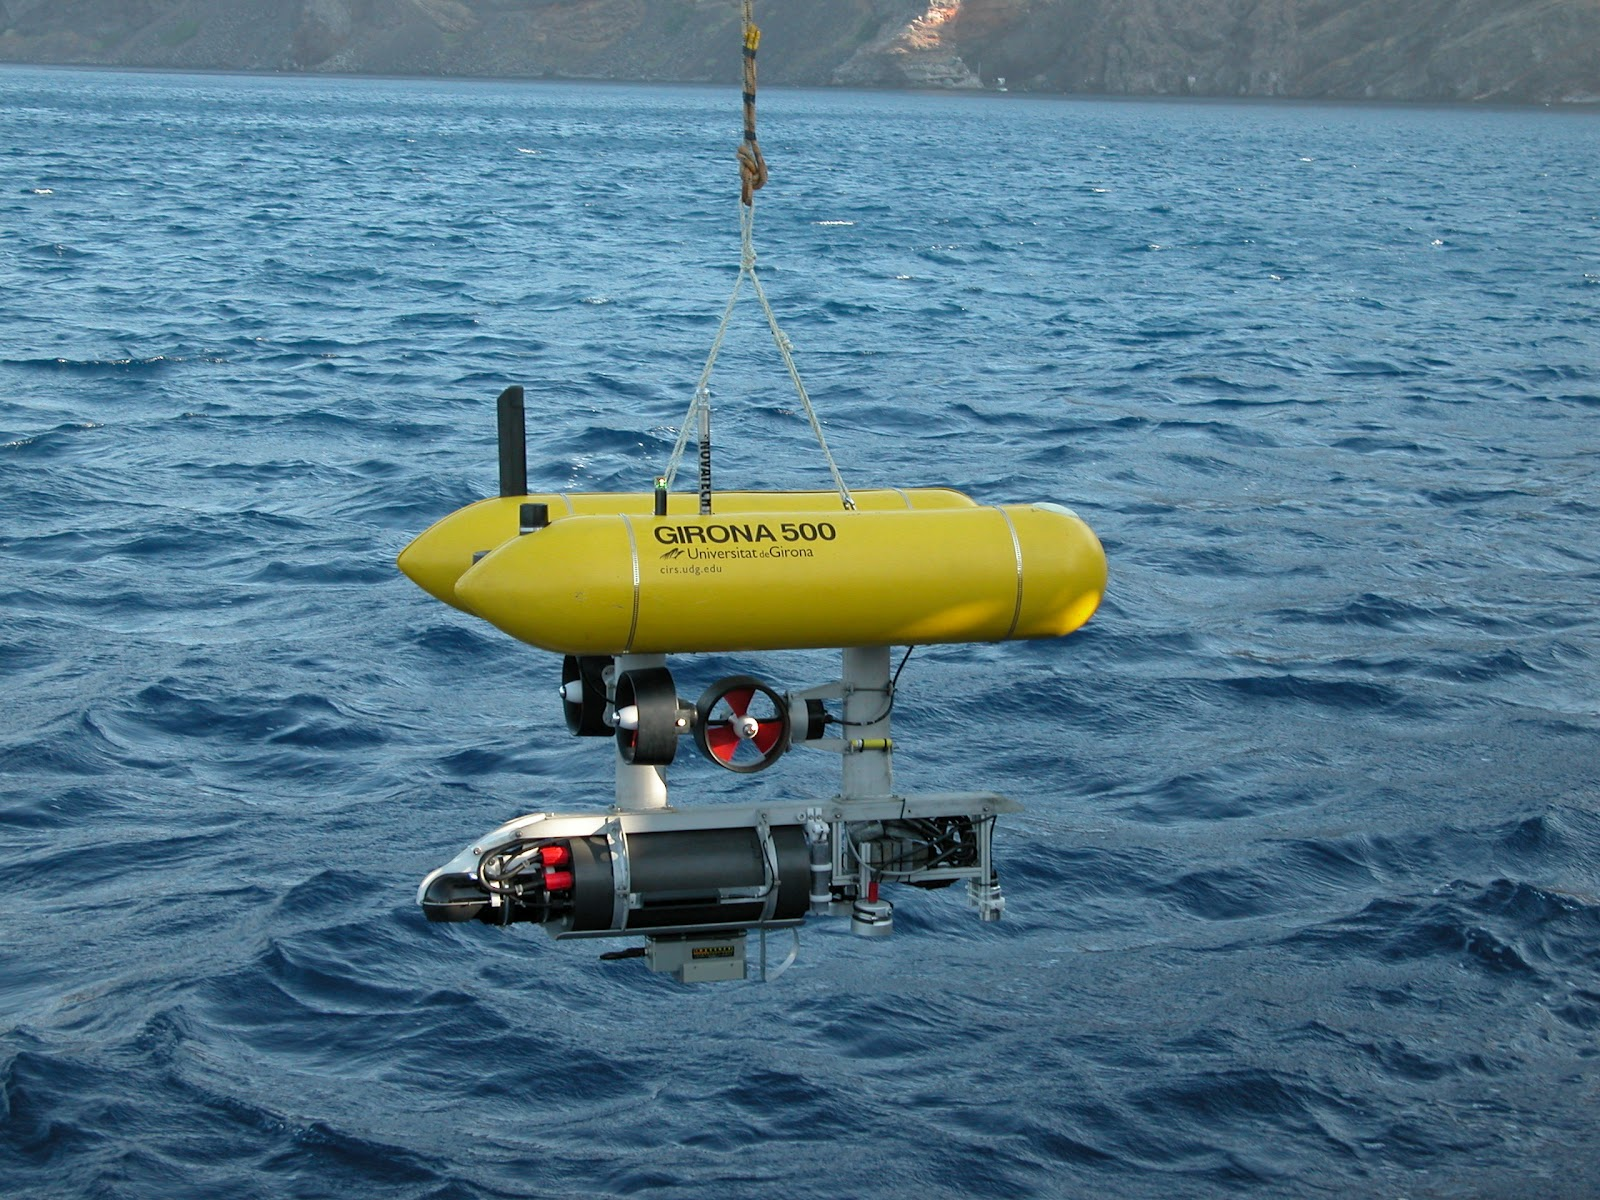
\includegraphics[width=\textwidth]{assets/girona500.jpg}
\caption{The Girona 500 AUV, equipped with an Inertial Navigation System (INS), facilitates geometric cross-modal co-registration.}
\label{fig:girona500}
\end{figure}

Establishing pixel-level correspondence between side-scan sonar (SSS) and optical imagery is challenging due to disparate sensor geometries, altitudes, and physical modalities. To enable robust cross-modal feature registration, we propose a geometry-driven pipeline that reconstructs a shared 3D spatial representation.

Following data acquisition via a dense, high-overlap lawnmower survey, we process the optical imagery using Structure-from-Motion (SfM). The resulting dense 3D seafloor mesh serves as the geometric ground truth bridging the visual and acoustic domains.

\subsection{Physics-Guided Reflectivity Isolation}
We map raw SSS intensities onto the 3D mesh to isolate intrinsic seabed acoustic properties. Under a Lambertian reflection model, raw acoustic intensity is $I = \rho \cos(\theta) L$, where $\rho$ is seabed reflectivity, $\theta$ is the local incidence angle, and $L$ is acoustic propagation loss. 

Because the SfM mesh provides high-fidelity 3D geometry, we calculate $\theta$ using local surface normals and computationally remove geometric view-dependence by dividing the recorded intensity by $\cos(\theta)$. Furthermore, because slant range is constant along each SSS waterfall column $C$, propagation loss $L$ is constant for any bins $b_i, b_j$ within that column:
\begin{equation}
   \forall b_i, b_j \in C, \; L(b_i) = L(b_j)
\end{equation}
By dividing each column by its average intensity, we factor out slant-dependent effects to yield normalized, relative reflectivity values. 

Finally, we wrap this isolated acoustic reflectivity texture alongside the optical RGB texture over the 3D mesh. Rendering the scene from arbitrary virtual camera poses allows us to rapidly curate a vast dataset of strictly co-registered, pixel-to-pixel optical and SSS image pairs.

\section{Methodology: Domain-Adaptive Self-Distillation}

Direct application of DINO-style self-distillation to side-scan sonar (SSS) imagery is challenging due to acoustic-specific statistics (speckle noise, gain variations) and small-batch distributed training constraints. We present a physics-informed self-distillation framework adapted to these conditions.

\subsection{Backbone and Initialization}
We employ ConvNeXt-tiny \cite{liu2022} as the backbone to extract multi-scale dense features, capturing both fine textures and broader semantic structures. Features are taken from stages $s \in \{2, 3, 4\}$ of the network, denoted $\mathbf{F}^{(s)} \in \mathbb{R}^{C_s \times H_s \times W_s}$.

The feature maps from stages 3 and 4 are upsampled to the resolution of stage 2 using bilinear interpolation:
\begin{equation}
\tilde{\mathbf{F}}^{(s)} = 
\begin{cases} 
\mathbf{F}^{(s)} & s = 2 \\
\mathcal{U}(\mathbf{F}^{(s)}, H_2, W_2) & s \in \{3, 4\}
\end{cases}
\end{equation}

Each upsampled map is $L_2$-normalized per spatial location:
\begin{equation}
\hat{\mathbf{f}}^{(s)}_{i,j} = \frac{\mathbf{f}^{(s)}_{i,j}}{\| \mathbf{f}^{(s)}_{i,j} \|_2 + \epsilon}
\end{equation}

The hypercolumn descriptor is formed by concatenation and final $L_2$ normalization:
\begin{equation}
\mathbf{H}_{i,j} = \text{Norm}\Bigl( \hat{\mathbf{f}}^{(2)}_{i,j} \oplus \hat{\mathbf{f}}^{(3)}_{i,j} \oplus \hat{\mathbf{f}}^{(4)}_{i,j} \Bigr)
\end{equation}
yielding a dense feature grid $\mathbf{H} \in \mathbb{R}^{D \times H_2 \times W_2}$.

For sub-pixel accuracy, we apply quadratic interpolation around each candidate match location using the second-order Taylor expansion of the local feature response, following the approach used in SIFT \cite{lowe2004}. Given that the final hypercolumn descriptors are normalized to lie on the unit hyper-sphere, the dot product can be used to directly compute the cosine similarity for matching between descriptors.

Initial matches are filtered using a model fitting strategy. RANSAC estimates a projective homography $H^*$ that minimizes reprojection error:
\begin{equation}
\epsilon = \| \mathbf{p}_{\text{fix}} - \pi(H \mathbf{p}_{\text{mov}}) \|_2^2
\end{equation}
retaining geometrically consistent inliers \cite{can2025_sss, katrusha2025}.

\subsection{The BenthiCat Dataset}

\begin{figure}[h]
\centering
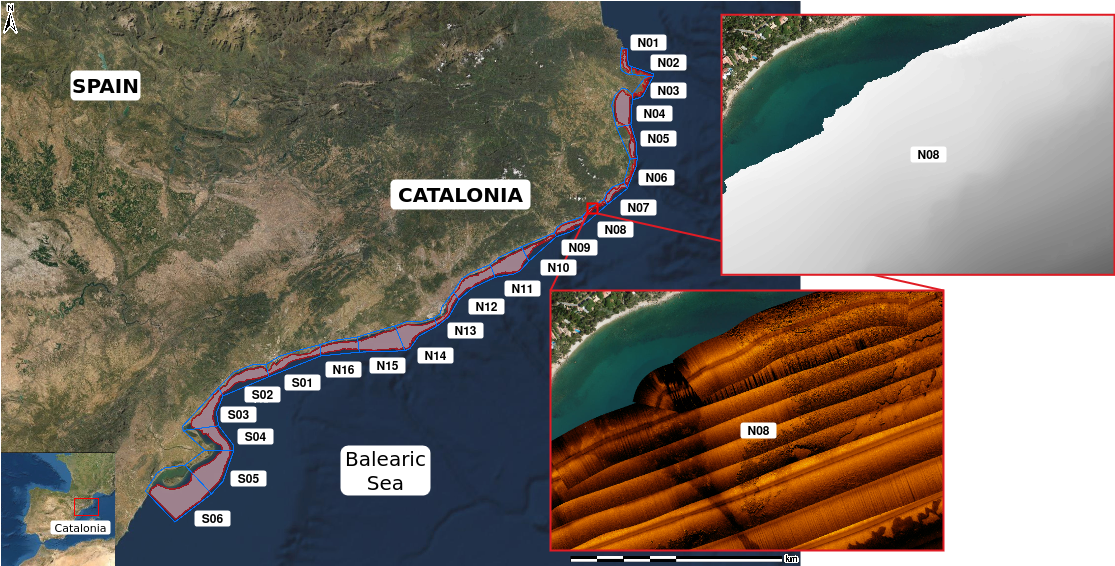
\includegraphics[width=\textwidth]{assets/benthicat.png}
\caption{The survey area of which the BenthiCat dataset was curated from.}
\label{fig:benthicat}
\end{figure}

The \textit{BenthiCat} dataset supports benthic habitat mapping with co-registered opti-acoustic data collected along the Catalan coast, covering $>1900\,\mathrm{km}^2$ \cite{hayat2025}. Acoustic data were acquired using a dual-frequency Klein 3000H SSS at $500\,\mathrm{kHz}$, achieving $\sim$8.5\,cm average slant-range resolution \cite{hayat2025,can2025_physdnet}.

It contains $\sim$1 million unannotated SSS image tiles suitable for self-supervised pre-training with DINOv3 \cite{hayat2025,oriane2025}. For supervised evaluation and fine-tuning, $\sim$36,000 tiles are annotated with pixel-wise segmentation masks across 12 habitat classes (e.g., \textit{Posidonia oceanica}, sand ripples, rock outcrops) \cite{hayat2025}.

Additionally, $178,000$ co-registered optical images were captured by the Girona1000 AUV at low altitude ($3.5$--$4.5\,\mathrm{m}$), georeferenced to corresponding SSS tiles. This enables cross-modal learning and verification of acoustic features against optical ground truth \cite{hayat2025}.

\subsubsection{Data Preprocessing}

\begin{figure}[h]
\centering
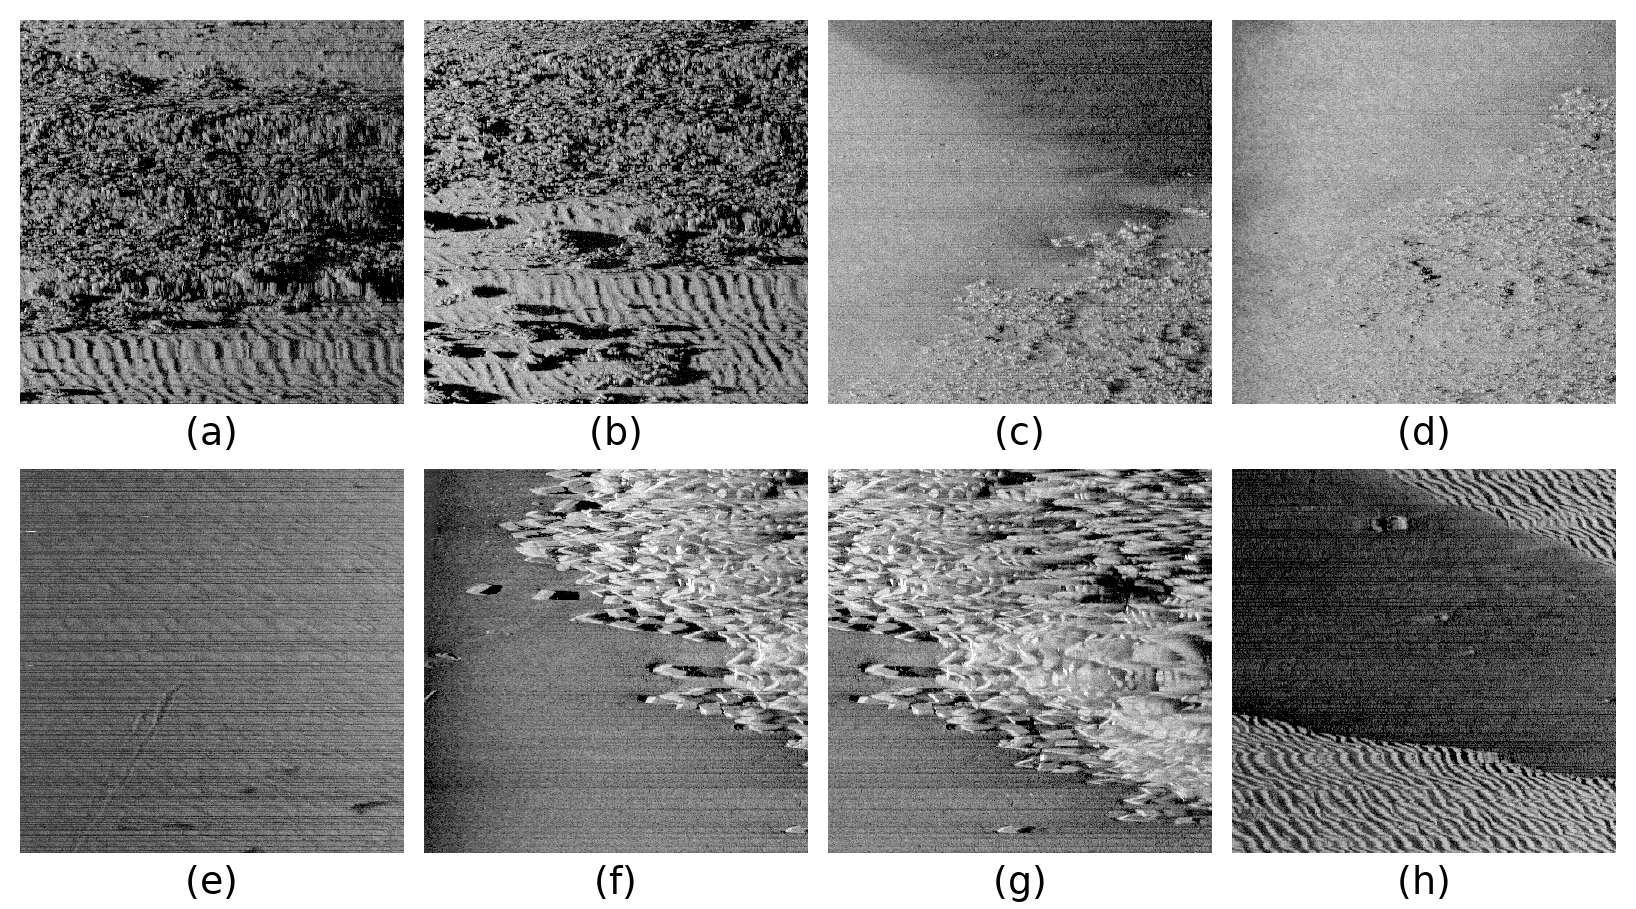
\includegraphics[width=\textwidth]{assets/samples.png}
\caption{Processed samples from the BenthiCat dataset.}
\label{fig:benthicat_samples}
\end{figure}

The raw 12-bit SSS waterfall data undergo several preprocessing steps. First, the data are subjected to logarithmic compression and normalization to between $[0,1]$ to stabilize training and preserve low-intensity detail:
\begin{equation}
I'_{\mathrm{normalized}} = \frac{\ln(1 + I_{\mathrm{raw}})}{\max(\ln(1 + I_{\mathrm{raw}}))}.
\end{equation}
Next, slant-range correction is applied under the flat-floor assumption to convert slant range $r_s$ to ground range $r_g$:
\begin{equation}
r_g = \sqrt{r_s^2 - h^2},
\end{equation}
which removes the nadir compression and blind zone \cite{antoni2016,hayat2025}. Finally, the data are tiled into overlapping $384 \times 384$ pixel patches with a 192-pixel stride in both along- and across-track directions to preserve structural continuity and leverage ConvNeXt translation equivariance \cite{liu2022,hayat2025}.

\subsection{Physics-Guided Augmentations}
To ensure feature invariance against common acoustic artifacts, we applied three physically motivated data augmentations. First, to simulate the speckle noise inherent in acoustic imagery \cite{alan2022}, we injected Gaussian noise into the input tiles. This acts as a denoising regularizer that forces the network to learn robust structural representations \cite{alan2022}.

Second, to account for uncompensated transmission loss, we applied synthetic Time-Varying Gain (TVG) profiles. By artificially injecting varied range-dependent attenuation curves \cite{antoni2016}, we compel the network to learn range-invariant features decoupled from physical acoustic attenuation.

Finally, to simulate dynamic range variations caused by operator adjustments or automatic gain control (AGC) \cite{antoni2016}, we applied random color jitter. Perturbing the brightness and contrast ensures invariance to radiometric calibration errors, driving the network to focus on intrinsic seabed reflectivity $\rho$ rather than transient intensity scaling \cite{can2025_sss}.

\subsection{Multi-Modal Feature Matching}
As previously discussed, a geometrically aligned opti-acoustic dataset can be effictively leveraged to learn a cross-modal matching function. Dense acoustic features are extracted from the synthetic reflectivity images using the fully trained, view-invariant ConvNeXt-DINOv3 backbone. Simultaneously, optical features are extracted from the corresponding RGB images. We then train a Multi-Layer Perceptron (MLP) to project the optical features into the acoustic feature space. The MLP learns the complex, non-linear mapping between photometric appearance and acoustic backscatter, ultimately allowing the system to robustly match optical features directly with extracted sonar features for high-precision, cross-modal localization and registration.

\subsection{Training Stabilisation and Loss Modifications}
Training runs on two NVIDIA Quadro RTX 6000 GPUs with an effective batch size of 170 (85 per GPU $\times$ 2 views). The original DINOv3 high-dimensional output ($K=65{,}536$) caused near-zero gradients due to the relatively small batch sizes. As such, we reduced the projection head output to $K=128$ to ensure meaningful prototype occupancy and stable gradients.

The Sinkhorn-Knopp algorithm in the DINO loss frequently produced zero rows/columns, leading to NaNs. We replaced it with the DINOv1 centering mechanism for the global-to-local distillation loss \cite{caron2021}:
\begin{equation}
    C_{t} \leftarrow m C_{t-1} + (1-m) \frac{1}{B} \sum_{i=1}^{B} O_{\text{teacher}}(x_i)
\end{equation}
The teacher output center $C$ is subtracted before softmax. This prevents collapse without Sinkhorn's strict constraints. The iBOT masked image modeling head retains Sinkhorn, as patch tokens provide sufficient density.

\section{Results and Discussion}

\subsection{Self-Supervised Learning using DINO}

\begin{figure}[htbp]
  \centering
  \begin{tabular}{c c c c}
    \begin{subfigure}[b]{0.24\linewidth}
      \centering
      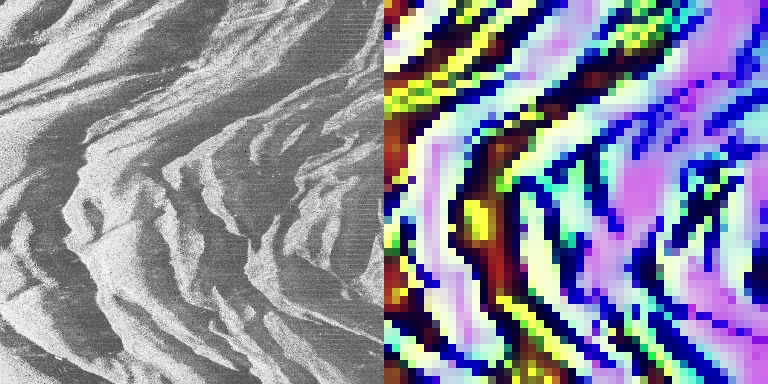
\includegraphics[width=\linewidth]{results/dino/dino0.jpeg}
    \end{subfigure}
    &
    \begin{subfigure}[b]{0.24\linewidth}
      \centering
      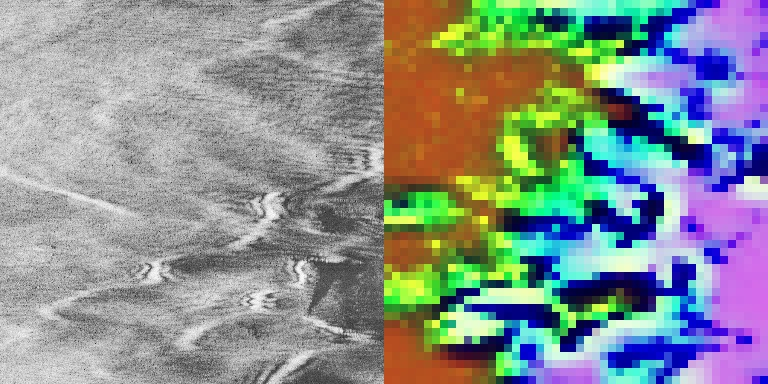
\includegraphics[width=\linewidth]{results/dino/dino1.jpeg}
    \end{subfigure}
    &
    \begin{subfigure}[b]{0.24\linewidth}
      \centering
      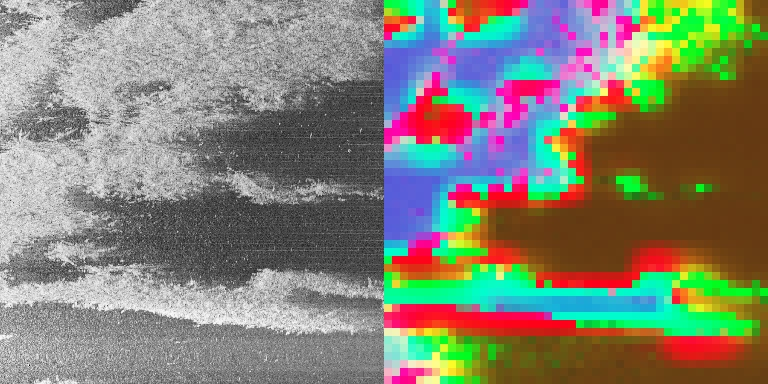
\includegraphics[width=\linewidth]{results/dino/dino2.jpeg}
    \end{subfigure}
    &
    \begin{subfigure}[b]{0.24\linewidth}
      \centering
      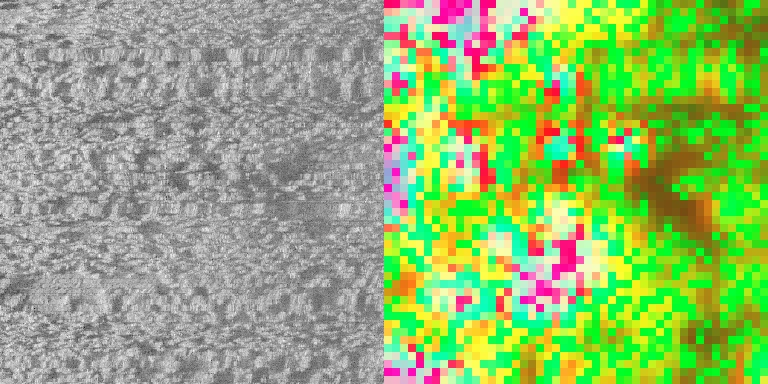
\includegraphics[width=\linewidth]{results/dino/dino3.jpeg}
    \end{subfigure}
    \\[6pt]
    \begin{subfigure}[b]{0.24\linewidth}
      \centering
      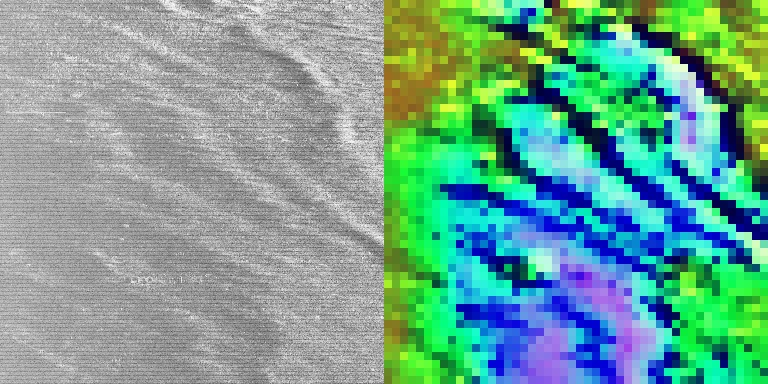
\includegraphics[width=\linewidth]{results/dino/dino4.jpeg}
    \end{subfigure}
    &
    \begin{subfigure}[b]{0.24\linewidth}
      \centering
      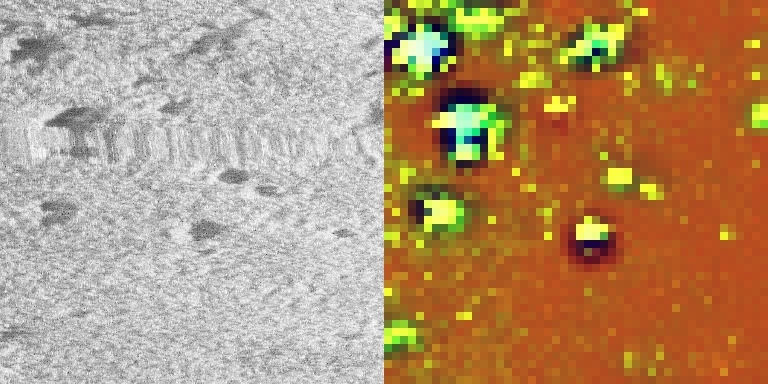
\includegraphics[width=\linewidth]{results/dino/dino5.jpeg}
    \end{subfigure}
    &
    \begin{subfigure}[b]{0.24\linewidth}
      \centering
      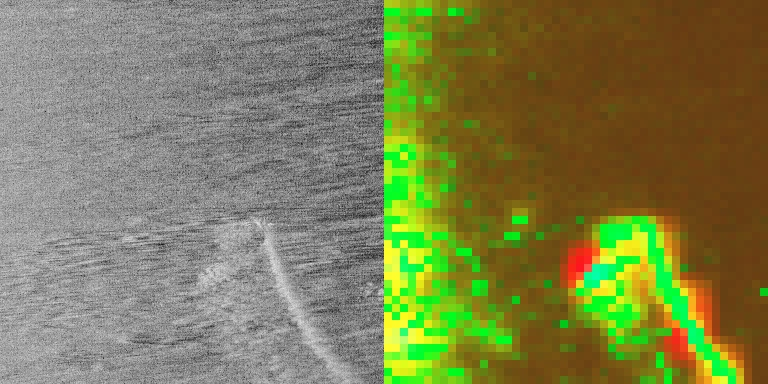
\includegraphics[width=\linewidth]{results/dino/dino6.jpeg}
    \end{subfigure}
    &
    \begin{subfigure}[b]{0.24\linewidth}
      \centering
      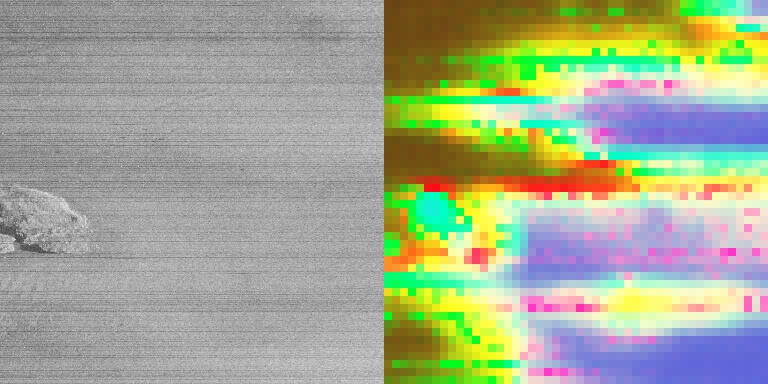
\includegraphics[width=\linewidth]{results/dino/dino7.jpeg}
    \end{subfigure}
  \end{tabular}
  \caption{Visualization of the outputted SSL semantic features by mapping the top three PCA components to RGB.}
  \label{fig:results_dino}
\end{figure}

Although architectural modifications and custom training protocols yielded visually coherent semantic features, full quantitative validation via ablation studies fell outside the time-constraints of this thesis. Instead, this section establishes the mathematical formulations for proposed ablation metrics to evaluate the robustness, dimensionality, and semantic depth of the learned feature space.

\subsubsection{Alignment vs. Uniformity}
Contrastive representation learning quality can be quantified by measuring feature alignment and uniformity on the unit hypersphere \cite{contrastive_ablation}. The alignment metric evaluates the expected distance between positive pairs:
\begin{equation}
\mathcal{L}_{\text{align}}(f; \alpha) \triangleq \mathbb{E}_{(x,y)\sim p_{\text{pos}}}\left[\|f(x) - f(y)\|^\alpha_2\right], \quad \alpha > 0
\end{equation}
where $\alpha=2$ conventionally \cite{contrastive_ablation}. 

Conversely, uniformity measures how evenly the feature distribution scales across the hypersphere to preserve maximal information:
\begin{equation}
\mathcal{L}_{\text{uniform}}(f; t) \triangleq \log \mathbb{E}_{x, y \sim p_{\text{data}}}\left[e^{-t\|f(x) - f(y)\|^2_2}\right], \quad t > 0
\end{equation}
where $t=2$ \cite{contrastive_ablation}. Low uniformity signifies representation collapse, indicating that the features lack semantic richness and fail to preserve data diversity.

\subsubsection{Singular Value Decomposition (SVD) of Features}
To diagnose dimensional collapse—where embedding vectors span only a lower-dimensional subspace—we analyze the variance of the feature space \cite{svd_ablation}. The covariance matrix $C \in \mathbb{R}^{d \times d}$ of $d$-dimensional embeddings $z_i$ over $N$ validation samples is defined as:
\begin{equation}
C = \frac{1}{N} \sum_{i=1}^N (z_i - \bar{z})(z_i - \bar{z})^T
\end{equation}
where $\bar{z}$ is the mean embedding \cite{svd_ablation}. Applying Singular Value Decomposition (SVD) yields $C = U S V^T$, where the diagonal matrix $S$ contains the sorted singular values $\sigma_k$. 

A rapid, abrupt decay in a logarithmic plot ($\log(\sigma_k)$)—where the top two or three components capture $\ge 90\%$ of the variance—indicates that the model exploits trivial global features (e.g., average backscatter intensity). Conversely, a gradually decaying, well-distributed spectrum across all dimensions confirms a rich, high-dimensional feature set.

\subsubsection{Silhouette Score}
The Silhouette score quantifies cluster distinctness and structural separation following dense feature clustering (e.g., via $k$-means) \cite{silhoutte_ablation}. For a patch $i$ in cluster $A$, let $a(i)$ be its average intra-cluster dissimilarity. The inter-cluster separation $b(i)$ is the minimum average dissimilarity to any neighboring cluster $C$:
\begin{equation}
b(i) = \min_{C \neq A} d(i, C)
\end{equation}
The resulting silhouette coefficient $s(i)$ is bounded between -1 and 1:
\begin{equation}
s(i) = \frac{b(i) - a(i)}{\max\{a(i), b(i)\}}
\end{equation}
The global silhouette width is the mean $s(i)$ across the dataset. Scores approaching 1 indicate tight, well-separated semantic boundaries, validating feature richness \cite{silhoutte_ablation}.

\subsubsection{Nearest Neighbor Qualitative Ablation}
Unlike linear probing or fine-tuning, which introduce hyperparameter sensitivity (e.g., weight decay), $k$-Nearest Neighbors ($k$-NN) classification cleanly isolates feature discriminability using only a single hyperparameter, $k$ \cite{lee2023rethinking}. Furthermore, in-domain $k$-NN performance serves as a reliable proxy for out-of-domain downstream tasks \cite{marks2024closer}. 

Using a frozen pre-trained backbone, cosine similarity measures semantic capacity between an anchor patch and target patches \cite{lee2023rethinking, marks2024closer}. Retrieving the top-5 nearest neighbors for specific semantic anchors (e.g., shipwrecks, pipelines, boulders) reveals feature properties: retrieving class-consistent structures across disparate cruises demonstrates robust semantic abstraction, whereas retrieving patches based solely on identical backscatter brightness diagnoses collapse to a trivial intensity histogram.

\subsection{Supervised Ablation Studies on Labeled Data}
While unsupervised metrics quantify intrinsic geometric properties, evaluating downstream semantic applicability via labeled data is critical. Although implementing these supervised ablations fell outside the current project scope, the framework below outlines the planned methodology for future validation.

\subsubsection{Linear Probe vs. $k$-NN Classifier}
Evaluating frozen features via linear probing and $k$-Nearest Neighbors ($k$-NN) is the standard protocol for assessing representation quality \cite{lee2023rethinking}. This approach freezes the pre-trained backbone and evaluates two simple downstream classifiers on the extracted features \cite{marks2024closer}:
\begin{itemize}
    \item \textbf{$k$-NN Classifier:} Requires no training; it categorizes test sonar patches based on Euclidean or cosine distance in the embedding space \cite{caron2021}.
    \item \textbf{Linear Probe:} Trains a single linear layer (e.g., logistic regression) parameterized by weights $W$ and bias $b$ to minimize cross-entropy loss \cite{lee2023rethinking}.
\end{itemize}

Comparing these metrics isolates the intrinsic clusterability of the representations. Performance parity between the $k$-NN and linear probe confirms a cleanly separated, linearly separable feature space \cite{caron2021, marks2024closer}. This proves that the DINOv3 objective naturally clusters sonar concepts without supervised boundaries. Conversely, if the linear probe outperforms $k$-NN, the features are rich but lack strict geometric disentanglement, requiring linear weights to resolve variance \cite{lee2023rethinking, marks2024closer}.

\subsubsection{Resolution and Patch Size Impact (Dense Feature Ablation)}
Side-scan sonar (SSS) imagery exhibits extreme scale variance, with critical features ranging from fine-grained sand ripples to massive shipwrecks \cite{can2025_sss, antoni2016}. To evaluate how the model handles this variance, we ablate feature resolution using the ConvNeXt backbone, which extracts hierarchical feature maps $\mathbf{F}^{(s)} \in \mathbb{R}^{C_s \times H_s \times W_s}$ across multiple stages (strides 4, 8, 16, and 32) \cite{liu2022}, and DINOv3, which optimizes dense features at high resolutions \cite{oriane2025}.

By extracting feature maps from different ConvNeXt stages and training a simple linear segmenter or classifier \cite{oquab2024}, we can measure classification accuracy or mean Intersection over Union (mIoU) at each stage. This identifies which layers encode the richest features for specific scales \cite{oriane2025, oquab2024}. Superior performance in early stages indicates a reliance on fine sediment textures, whereas deeper layers signify dependence on global semantic context for object-level hazard detection \cite{liu2022, can2025_physdnet}.

\subsubsection{Data Efficiency (Few-Shot Scalability Curve)}
A robust self-supervised model must exhibit high data efficiency, particularly when labeled SSS data is scarce \cite{oriane2025, alan2022}. This efficiency can be quantified as an ablation metric by artificially restricting the training data available to the linear probe.

By training the linear classifier on restricted label subsets—specifically 1\%, 5\%, 10\%, 25\%, 50\%, and 100\%—we plot downstream performance against training data volume \cite{marks2024closer, caron2021}. A robust SSL model yields a flat few-shot scalability curve \cite{marks2024closer}. Achieving near-peak accuracy in low-data regimes (e.g., 1\% or 10\%) demonstrates that DINOv3 pre-training successfully captured generalizable representations, executing the bulk of feature learning prior to supervised fine-tuning \cite{marks2024closer}.

\subsection{Geometric Reconstruction Results and Calibration Challenges}

Vehicle Inertial Measurement Unit (IMU)-constrained Structure-from-Motion (SfM) was utilized to reconstruct 3D seafloor meshes. This approach yielded the precise localization and geometric accuracy necessary for mapping side-scan sonar data via the Lambertian reflection model.

However, the camera's nadir orientation and the lack of a calibrated sensor model introduced geometric artifacts. Because the SfM pipeline jointly estimated camera intrinsics and distortion parameters without a strict calibration prior, non-linear offsets occurred in the vehicle's estimated altitude relative to the seabed. Consequently, while the relative reconstructed geometry remained highly accurate, absolute depth and scale suffered from non-linearities.

These altitude offsets stem from two unconstrained optimization behaviors within the SfM solver:
\begin{itemize}
    \item \textbf{Dynamic Focal Length Estimation:} Jointly optimizing the focal length induced an artificial zooming effect, causing spatial errors to propagate non-linearly away from the optical center.
    \item \textbf{Unconstrained Radial Distortion:} Without physical constraints (e.g., an underwater calibration pattern), the solver converged to a local minimum. While this minimized reprojection errors, it failed to model water-column-induced radial distortions, thereby amplifying the altitude offsets.
\end{itemize}

\subsection{Altitude Offset Correction via First Bottom Return Extraction}

\begin{figure}[htbp]
  \centering
  \begin{tabular}{c c}
    \begin{subfigure}[b]{0.45\linewidth}
      \centering
      \includegraphics[width=\linewidth]{results/offset_correction/tile_before.png}
    \end{subfigure}
    &
    \begin{subfigure}[b]{0.45\linewidth}
      \centering
      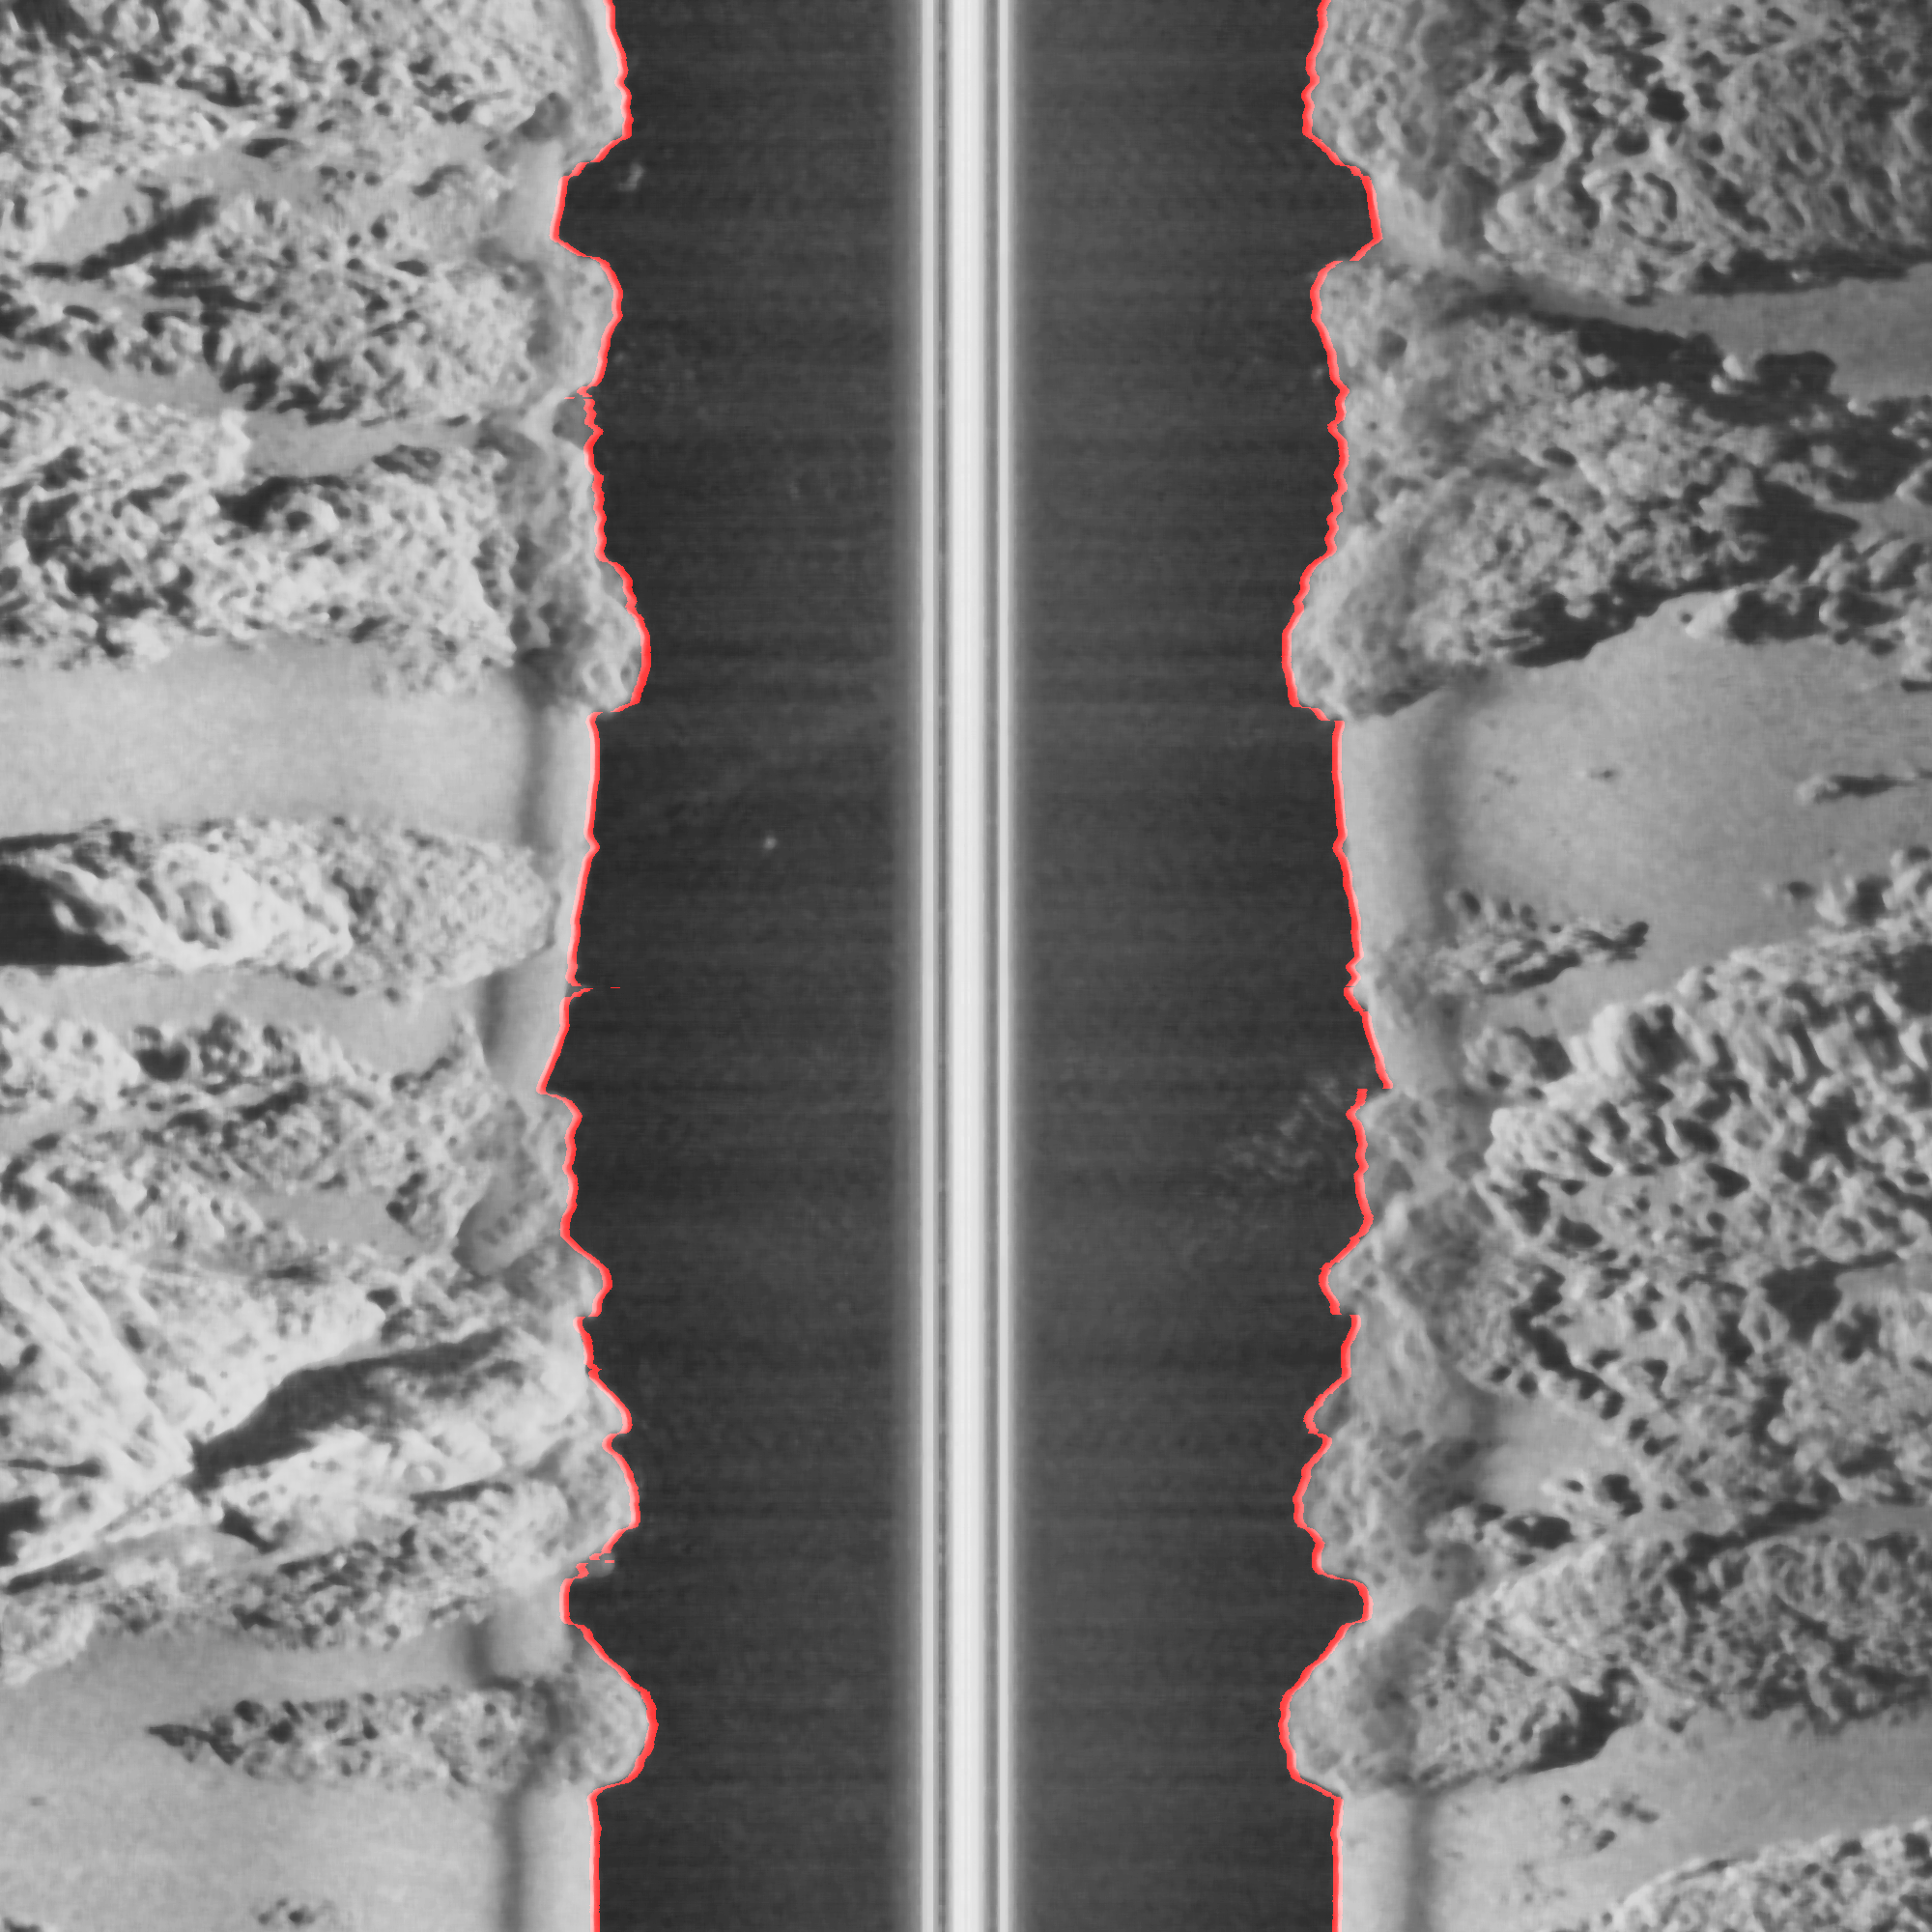
\includegraphics[width=\linewidth]{results/offset_correction/tile_first_return.png}
    \end{subfigure}
    \\[6pt]
    \begin{subfigure}[b]{0.45\linewidth}
      \centering
      \includegraphics[width=\linewidth]{results/offset_correction/tile_global.png}
    \end{subfigure}
    &
    \begin{subfigure}[b]{0.45\linewidth}
      \centering
      \includegraphics[width=\linewidth]{results/offset_correction/tile_local.png}
    \end{subfigure}
  \end{tabular}
  \caption{Top-left: Offset between SSS waterfall and geometry reprojection. Top-right: FBR detection performance. Bottom-left: After global offset correction. Bottom-right: After local offset correction. OpenCV's Rainbow colormap is applied to the relative acoustic reflectivity.}
  \label{fig:results_offset}
\end{figure}

To resolve non-linear altitude offsets from unconstrained geometric reconstruction, we present a localized correction method based on First Bottom Return (FBR) extraction from side-scan sonar (SSS) waterfall imagery. The FBR marks the first significant acoustic echo from the seafloor, delineating the water column and providing the true Autonomous Underwater Vehicle (AUV) altitude via its acoustic slant distance \cite{antoni2016}. 

First, raw port and starboard sonar channels are smoothed using a median filter to reduce speckle noise, followed by Contrast Limited Adaptive Histogram Equalization (CLAHE) to enhance edge contrast. A greedy algorithm then tracks the FBR by minimizing a cost function over a 100-bin sliding window:
\begin{equation}
\mathcal{C}(b) = 0.4 \cdot \nabla(b) + 0.3 \cdot \mathcal{D}_{\text{nadir}}(b) + 0.3 \cdot \mathcal{D}_{\text{past}}(b)
\end{equation}
where $\nabla(b)$ is the gradient magnitude at candidate bin $b$, $\mathcal{D}_{\text{nadir}}(b)$ is its spatial distance from the nadir, and $\mathcal{D}_{\text{past}}(b)$ is its distance relative to the FBR locations detected in the preceding $n$ bins. This formulation ensures temporal consistency across consecutive pings while capturing high-gradient seabed transitions.

The FBR-derived ground-truth altitude is then used to rectify the reconstructed 3D geometry. For each estimated AUV pose, the altitude offset is computed as the difference between this ground truth and the distance to the closest vertex in the reconstructed mesh. Global offset corrections across the entire trajectory fail to handle non-constant altitude errors and non-linear scaling artifacts caused by uncalibrated Structure-from-Motion (SfM). We address this by applying a dynamic, local offset correction. By computing the correction for any given pose using an adaptive temporal window of the 50 closest pings, the system successfully compensates for non-linear drift, achieving precise alignment between the waterfall imagery and its geometric reprojection (Fig. \ref{fig:results_offset}).

\subsection{Physics-Guided Reflectivity Isolation and Mesh Projection}

\begin{figure}[htbp]
  \centering
  \begin{subfigure}[b]{0.30\linewidth}
    \centering
    \includegraphics[width=\linewidth]{results/rocks/synthetic/orig.png}    
  \end{subfigure}
  \begin{subfigure}[b]{0.30\linewidth}
    \centering
    \includegraphics[width=\linewidth]{results/rocks/synthetic/over.png}
  \end{subfigure}
  \begin{subfigure}[b]{0.30\linewidth}
    \centering
    \includegraphics[width=\linewidth]{results/rocks/synthetic/synth.png}
  \end{subfigure}
  \caption{A patch from the SSS waterfall (left) along with its corresponding geometric reprojection (middle) and synthesized intensities based on the isolated reflectivity (right).}
  \label{fig:results_synthetic}
\end{figure}

To isolate the view-invariant material reflectivity ($\rho_v$), an inverse Lambertian reflection model is applied to the geometrically aligned side-scan sonar (SSS) waterfall and 3D mesh. The recorded backscatter intensity is modeled as a function of intrinsic seabed reflectivity, the cosine of the local incidence angle, and acoustic propagation loss.

\subsubsection{Geometric Projection and Shadow Filtering}
For each AUV pose, a projection plane is defined orthogonal to the along-track trajectory. Mesh vertices within a $5\text{ cm}$ radius of this plane are evaluated via raytracing; vertices with occluded lines-of-sight to the transducer are classified as acoustic shadows and discarded. 

Valid vertices are mapped to specific SSS waterfall bins based on their slant distance and transducer side (port/starboard). If multiple vertices project to the same bin, their local incidence angles ($\theta$) are averaged. The raw bin intensity is then divided by $\cos(\theta)$ to remove Lambertian geometric dependence. To eliminate slant-dependent propagation loss, each along-track column is normalized by its mean intensity, yielding a relative reflectivity $\rho_i$ for each bin.

\subsubsection{Physical Weighting and Blending}

\begin{figure}[htbp]
  \centering
  \begin{subfigure}[b]{0.45\linewidth}
    \centering
    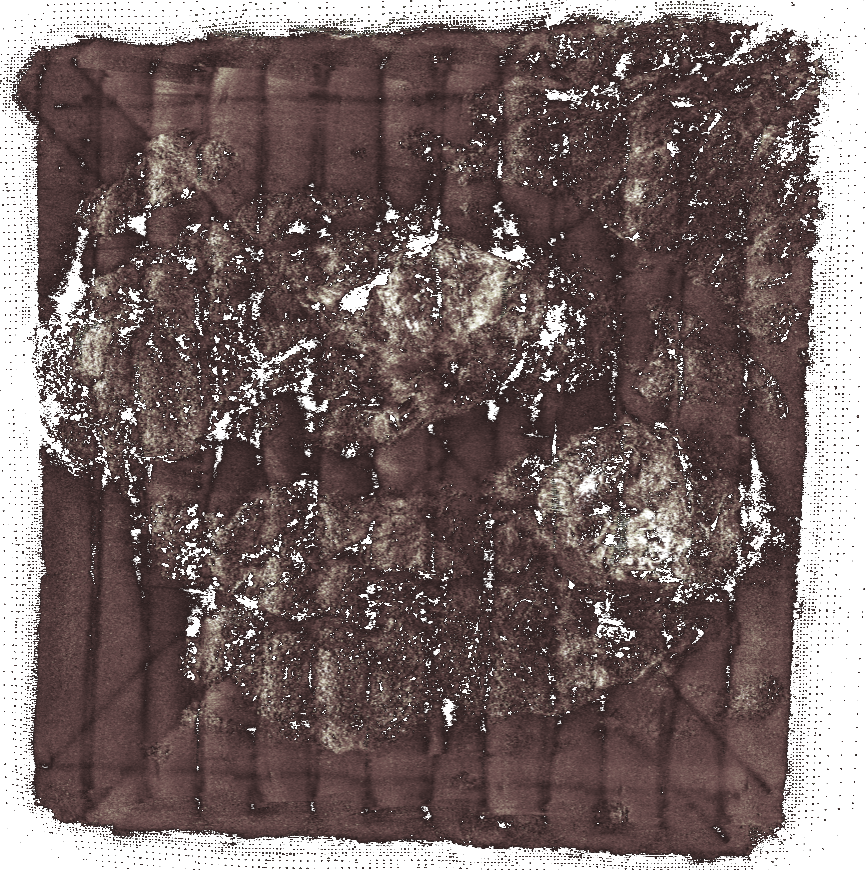
\includegraphics[width=\linewidth]{results/rocks/ref_mesh.png}    
  \end{subfigure}
  \begin{subfigure}[b]{0.45\linewidth}
    \centering
    
\includegraphics[width=\linewidth]{results/seagrass/ref_mesh.png}
  \end{subfigure}
  \caption{Reflectivity values of a mountaineous region mesh (left) and a seagrass region mesh (right). Brighter areas imply higher seabed reflectivity.}
  \label{fig:results_synthetic}
\end{figure}

The relative reflectivity values are projected back onto the 3D mesh using a dual-Gaussian weighting function, $\mathcal{W}(\theta, r_s)$, which models the sonar's emission physics and angular sensitivity:
\begin{equation}
\mathcal{W}(\theta, r_s) = \exp\left( - \frac{(\theta - \pi/4)^2}{2(\pi/16)^2} \right) \cdot \exp\left( - \frac{r_s^2}{2(12)^2} \right)
\end{equation}
where the first term weights the reflectivity by the incidence angle $\theta$ (centered at $\pi/4$ with a standard deviation of $\pi/16$), and the second term accounts for water-column energy attenuation across the slant distance $r_s$ (centered at zero with a standard deviation of $12\text{ m}$).

The final view-invariant reflectivity $\rho_{v}$ for each vertex is computed as the weighted average of all $N$ overlapping mapped bins:
\begin{equation}
\rho_{v} = \frac{\sum_{i=1}^{N} \mathcal{W}(\theta_i, r_{s,i}) \rho_i}{\sum_{i=1}^{N} \mathcal{W}(\theta_i, r_{s,i})}
\end{equation}

\subsection{Opti-Acoustic Co-Registration and Dataset Generation}

\begin{figure}[htbp]
  \centering
  \begin{tabular}{c c c}
    % \begin{subfigure}[b]{0.30\linewidth}
    %   \centering
    %   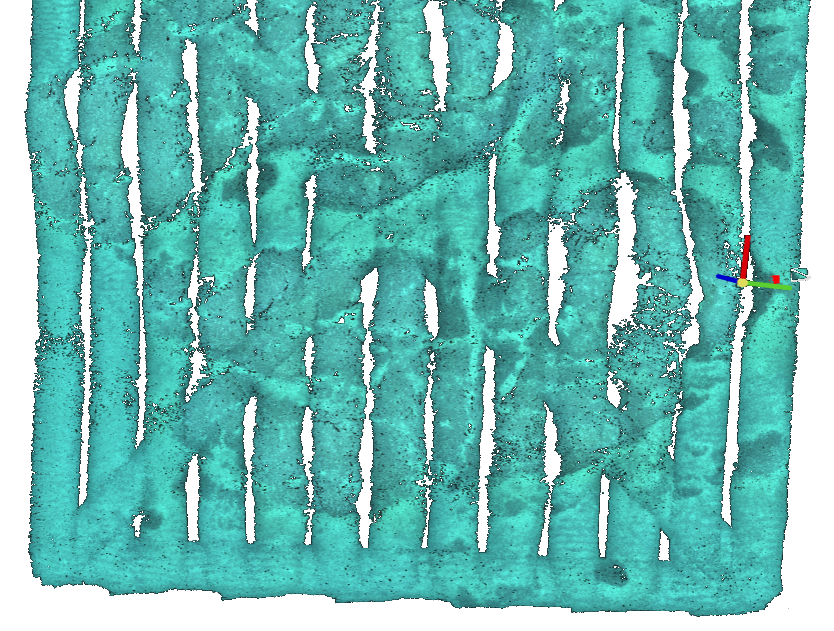
\includegraphics[width=\linewidth]{results/rocks/registration/pcd1.png}
    % \end{subfigure}
    % &
    % \begin{subfigure}[b]{0.30\linewidth}
    %   \centering
    %   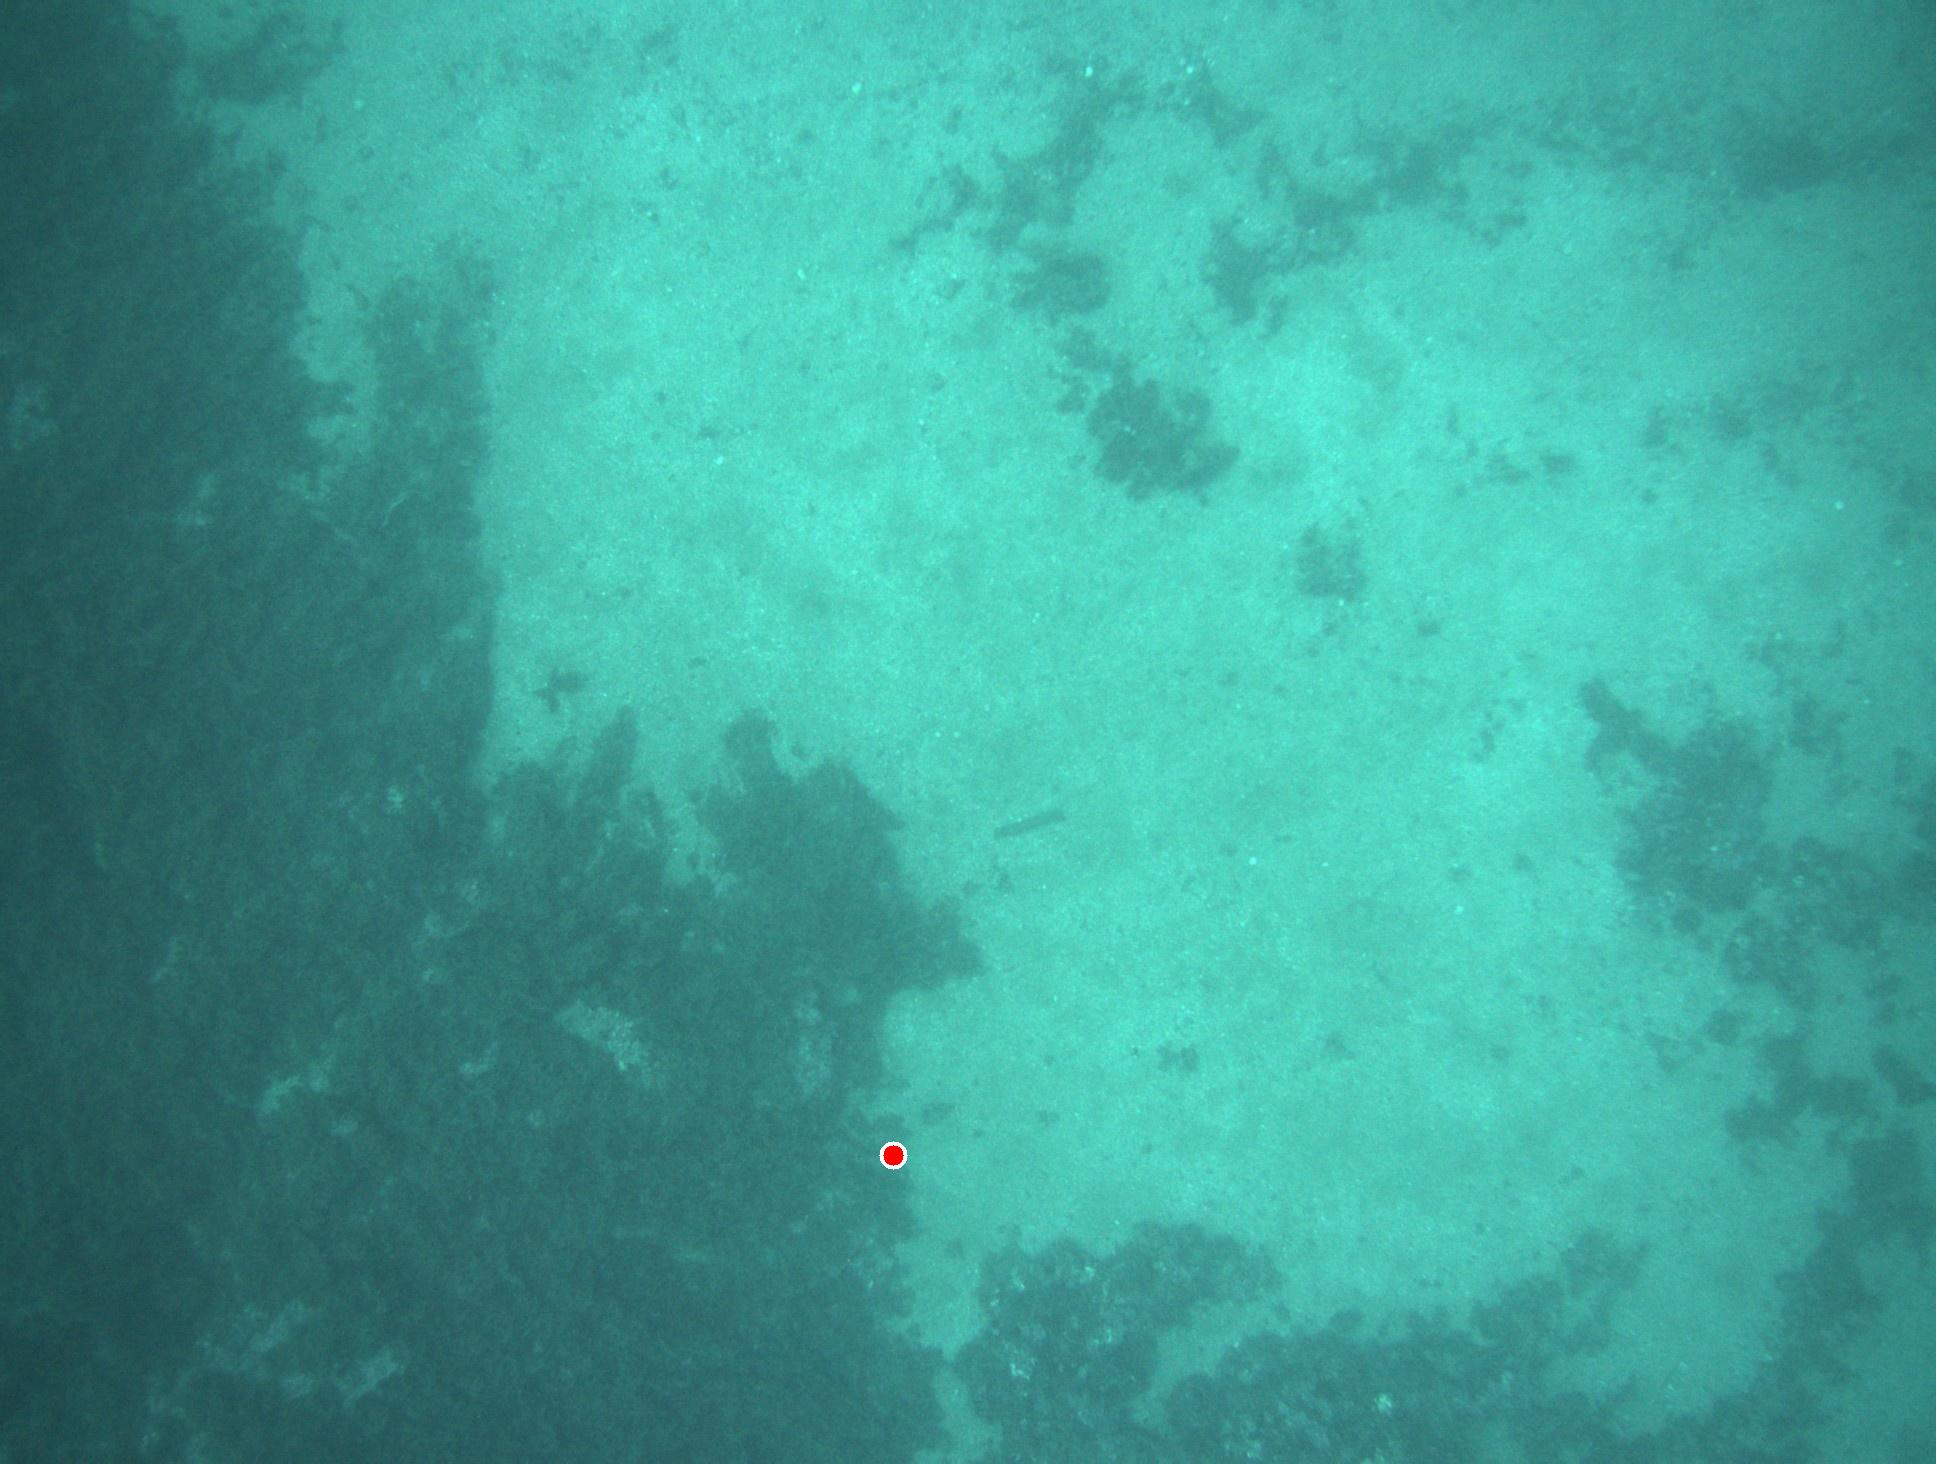
\includegraphics[width=\linewidth]{results/rocks/registration/optical1.jpeg}
    % \end{subfigure}
    % &
    % \begin{subfigure}[b]{0.30\linewidth}
    %   \centering
    %   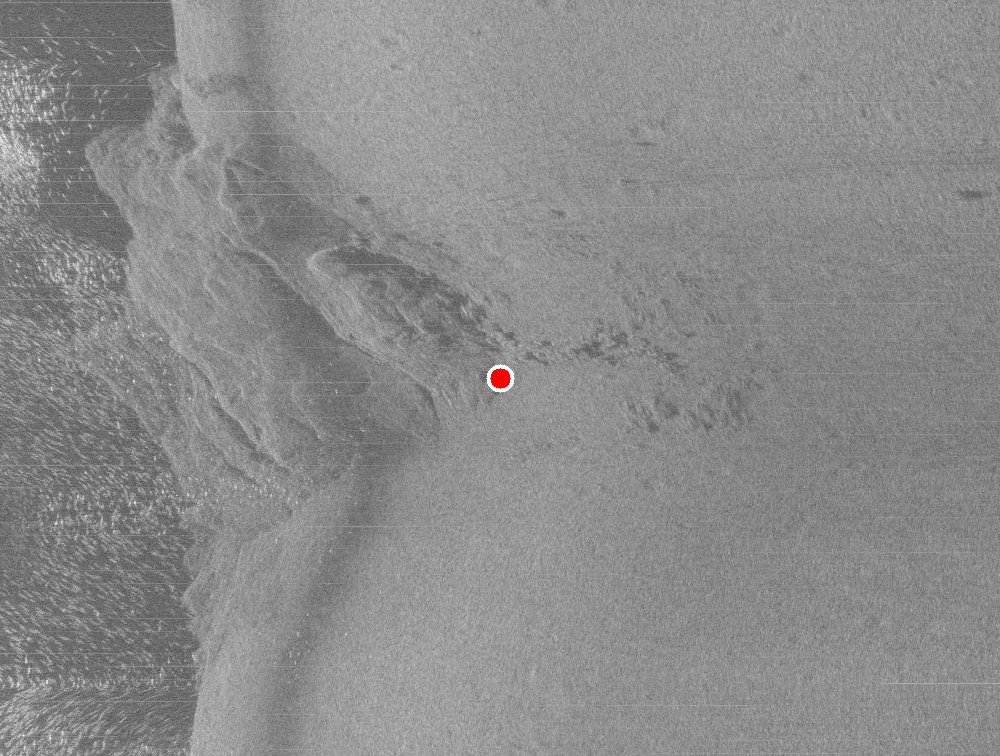
\includegraphics[width=\linewidth]{results/rocks/registration/sss1.jpeg}
    % \end{subfigure}
    % \\[6pt]
    \begin{subfigure}[b]{0.30\linewidth}
      \centering
      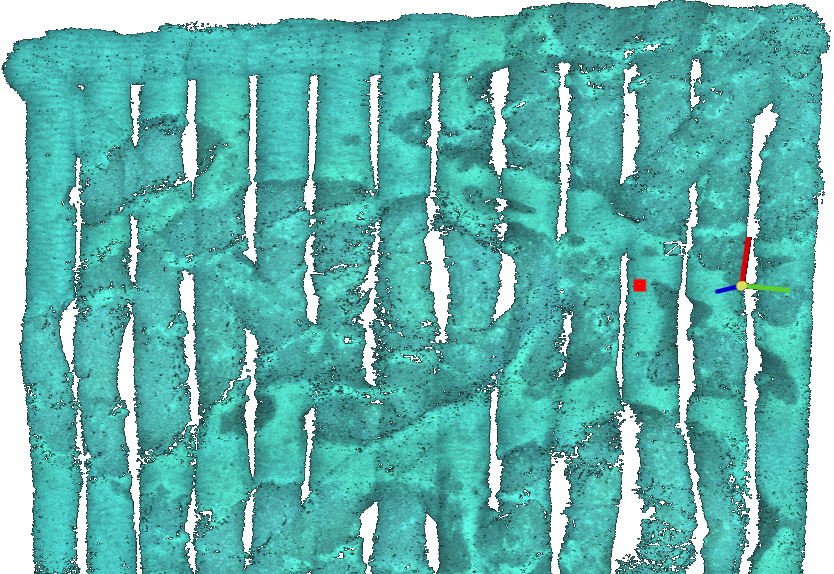
\includegraphics[width=\linewidth]{results/rocks/registration/pcd4.png}
    \end{subfigure}
    &
    \begin{subfigure}[b]{0.30\linewidth}
      \centering
      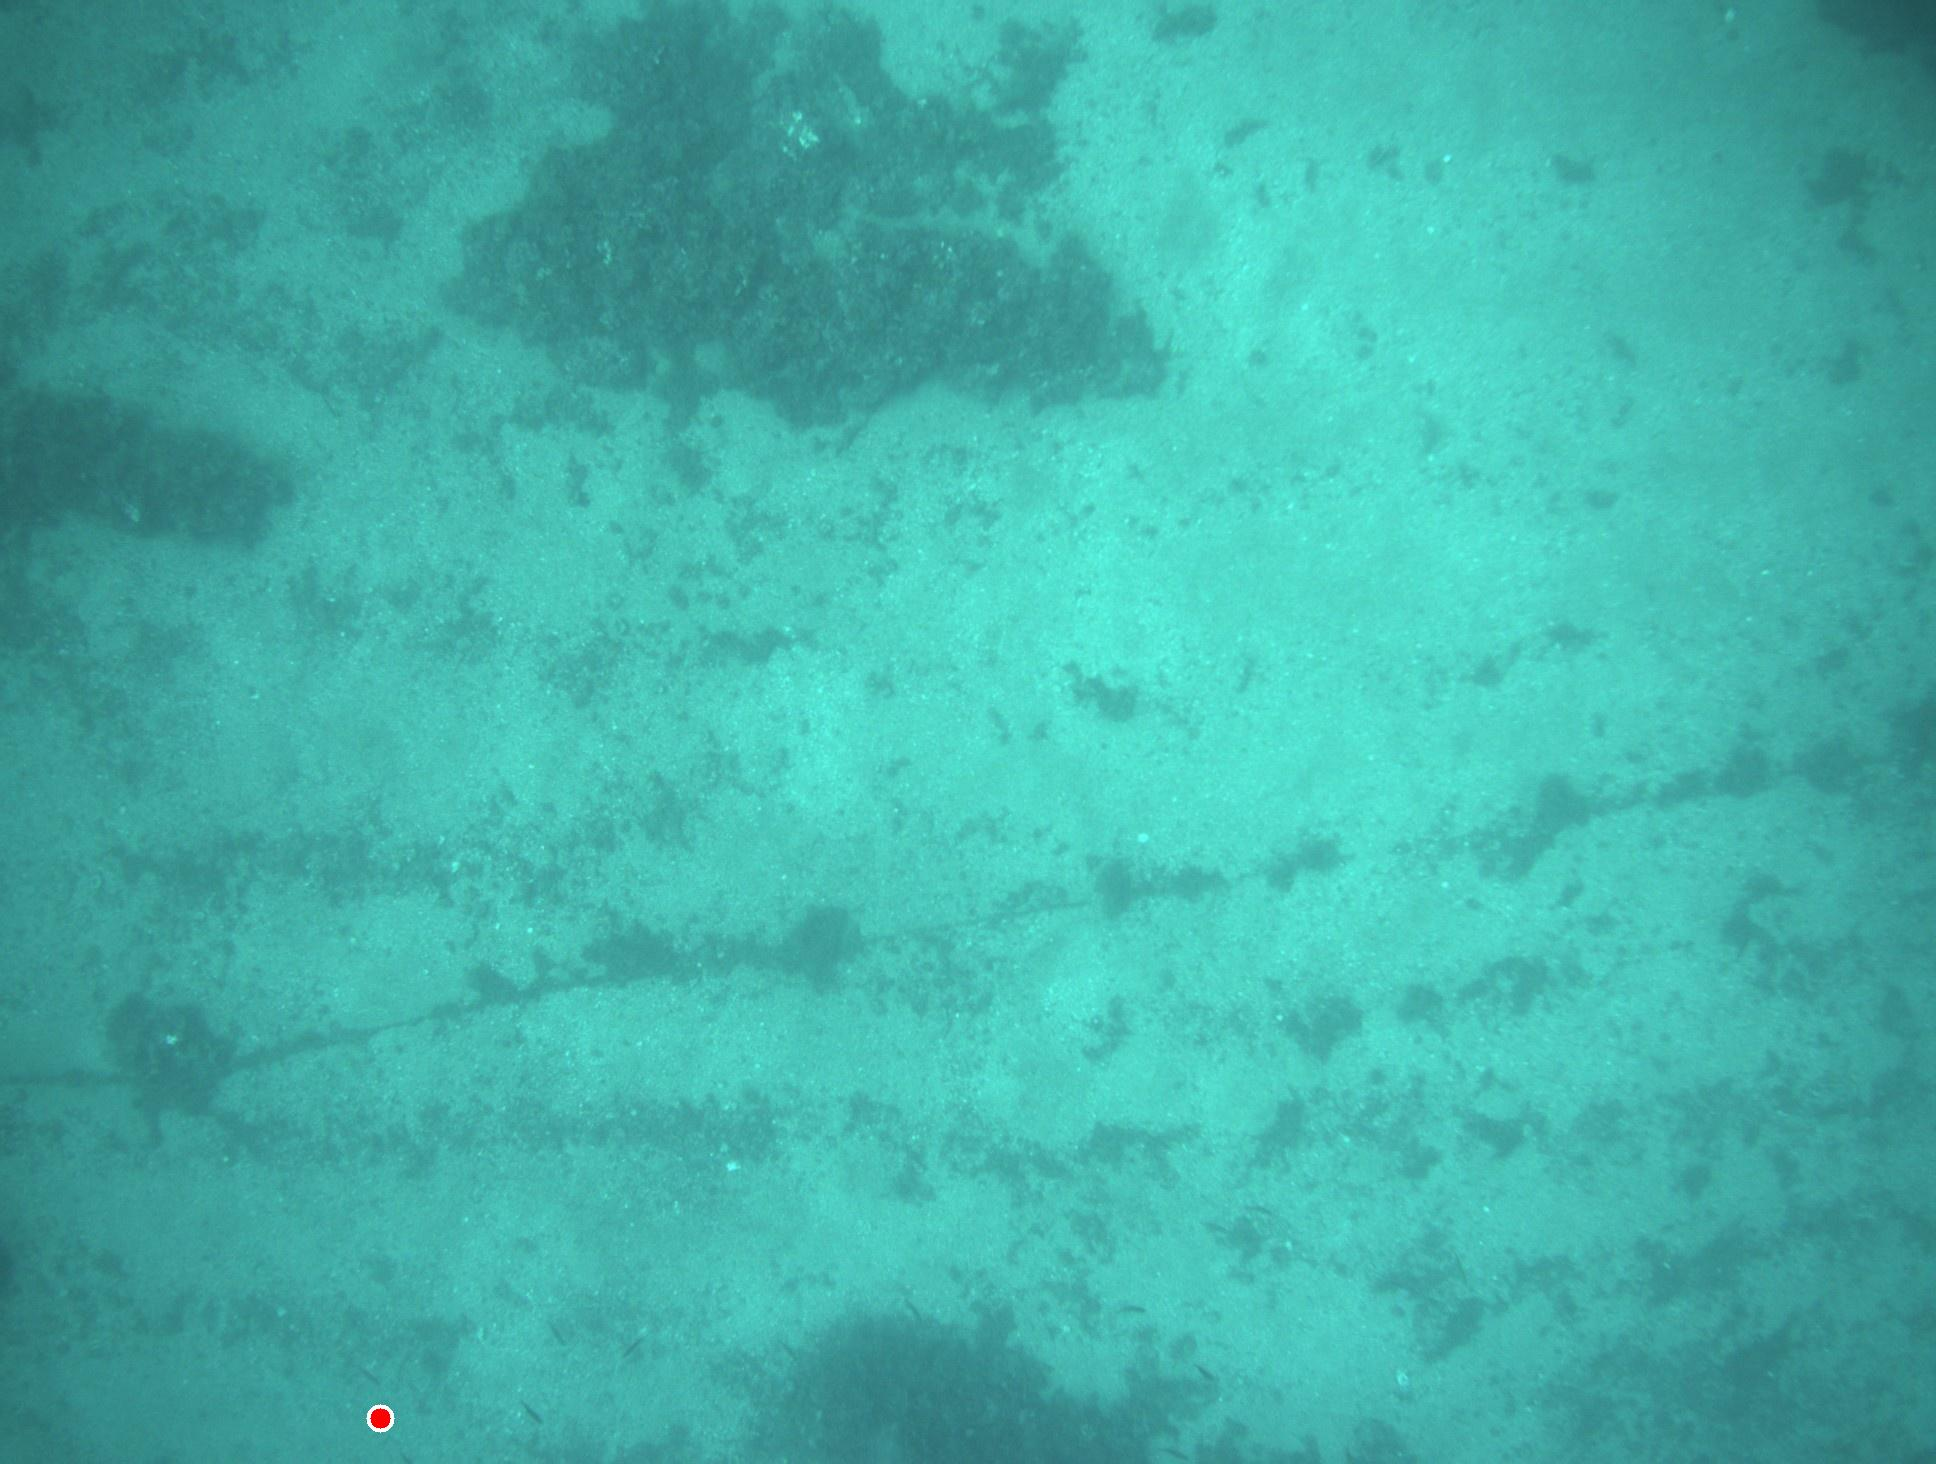
\includegraphics[width=\linewidth]{results/rocks/registration/optical4.jpeg}
    \end{subfigure}
    &
    \begin{subfigure}[b]{0.30\linewidth}
      \centering
      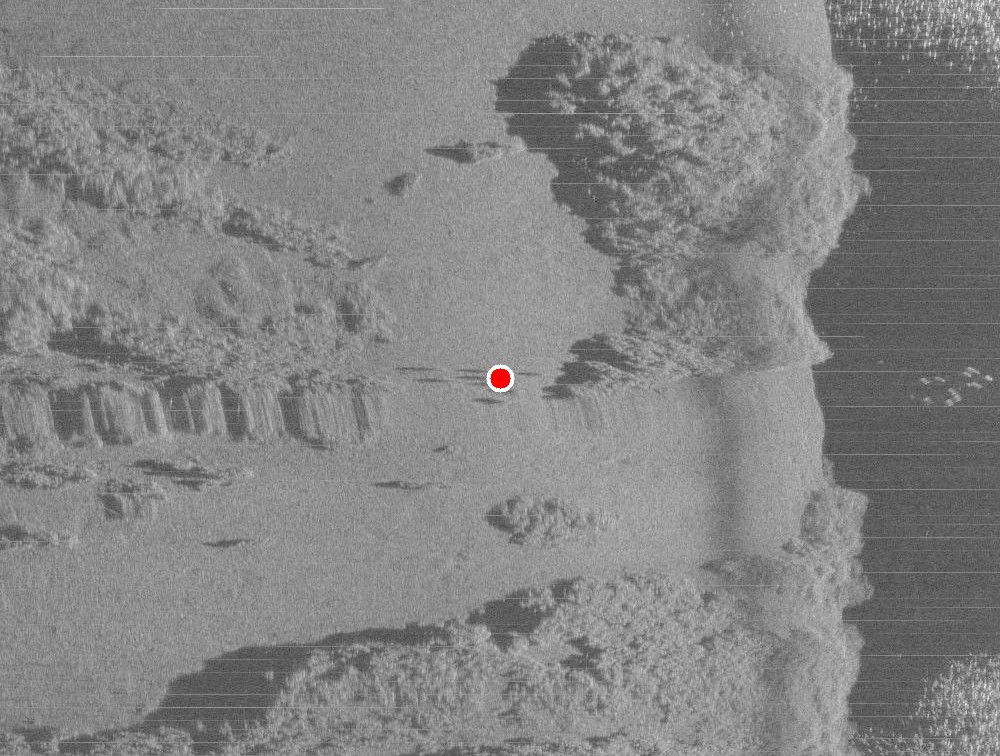
\includegraphics[width=\linewidth]{results/rocks/registration/sss4.jpeg}
    \end{subfigure}
    % \\[6pt]
    % \begin{subfigure}[b]{0.30\linewidth}
    %   \centering
    %   
\includegraphics[width=\linewidth]{results/seagrass/registration/pcd4.png}
    % \end{subfigure}
    % &
    % \begin{subfigure}[b]{0.30\linewidth}
    %   \centering
    %   
\includegraphics[width=\linewidth]{results/seagrass/registration/optical4.jpeg}
    % \end{subfigure}
    % &
    % \begin{subfigure}[b]{0.30\linewidth}
    %   \centering
    %   
\includegraphics[width=\linewidth]{results/seagrass/registration/sss4.jpeg}
    % \end{subfigure}
    \\[6pt]
    \begin{subfigure}[b]{0.30\linewidth}
      \centering
      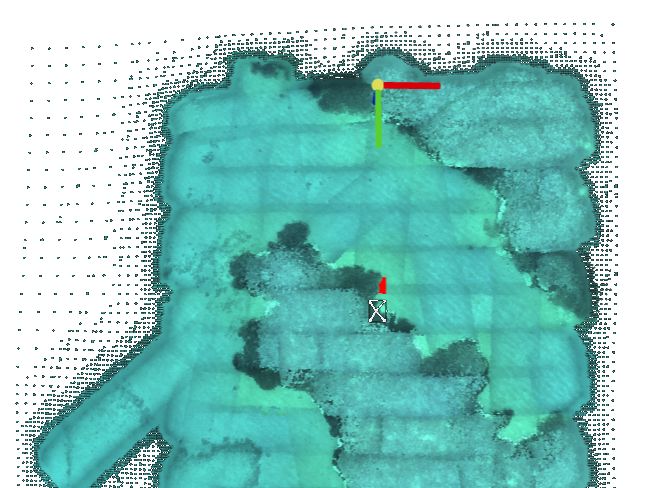
\includegraphics[width=\linewidth]{results/seagrass/registration/pcd5.png}
    \end{subfigure}
    &
    \begin{subfigure}[b]{0.30\linewidth}
      \centering
      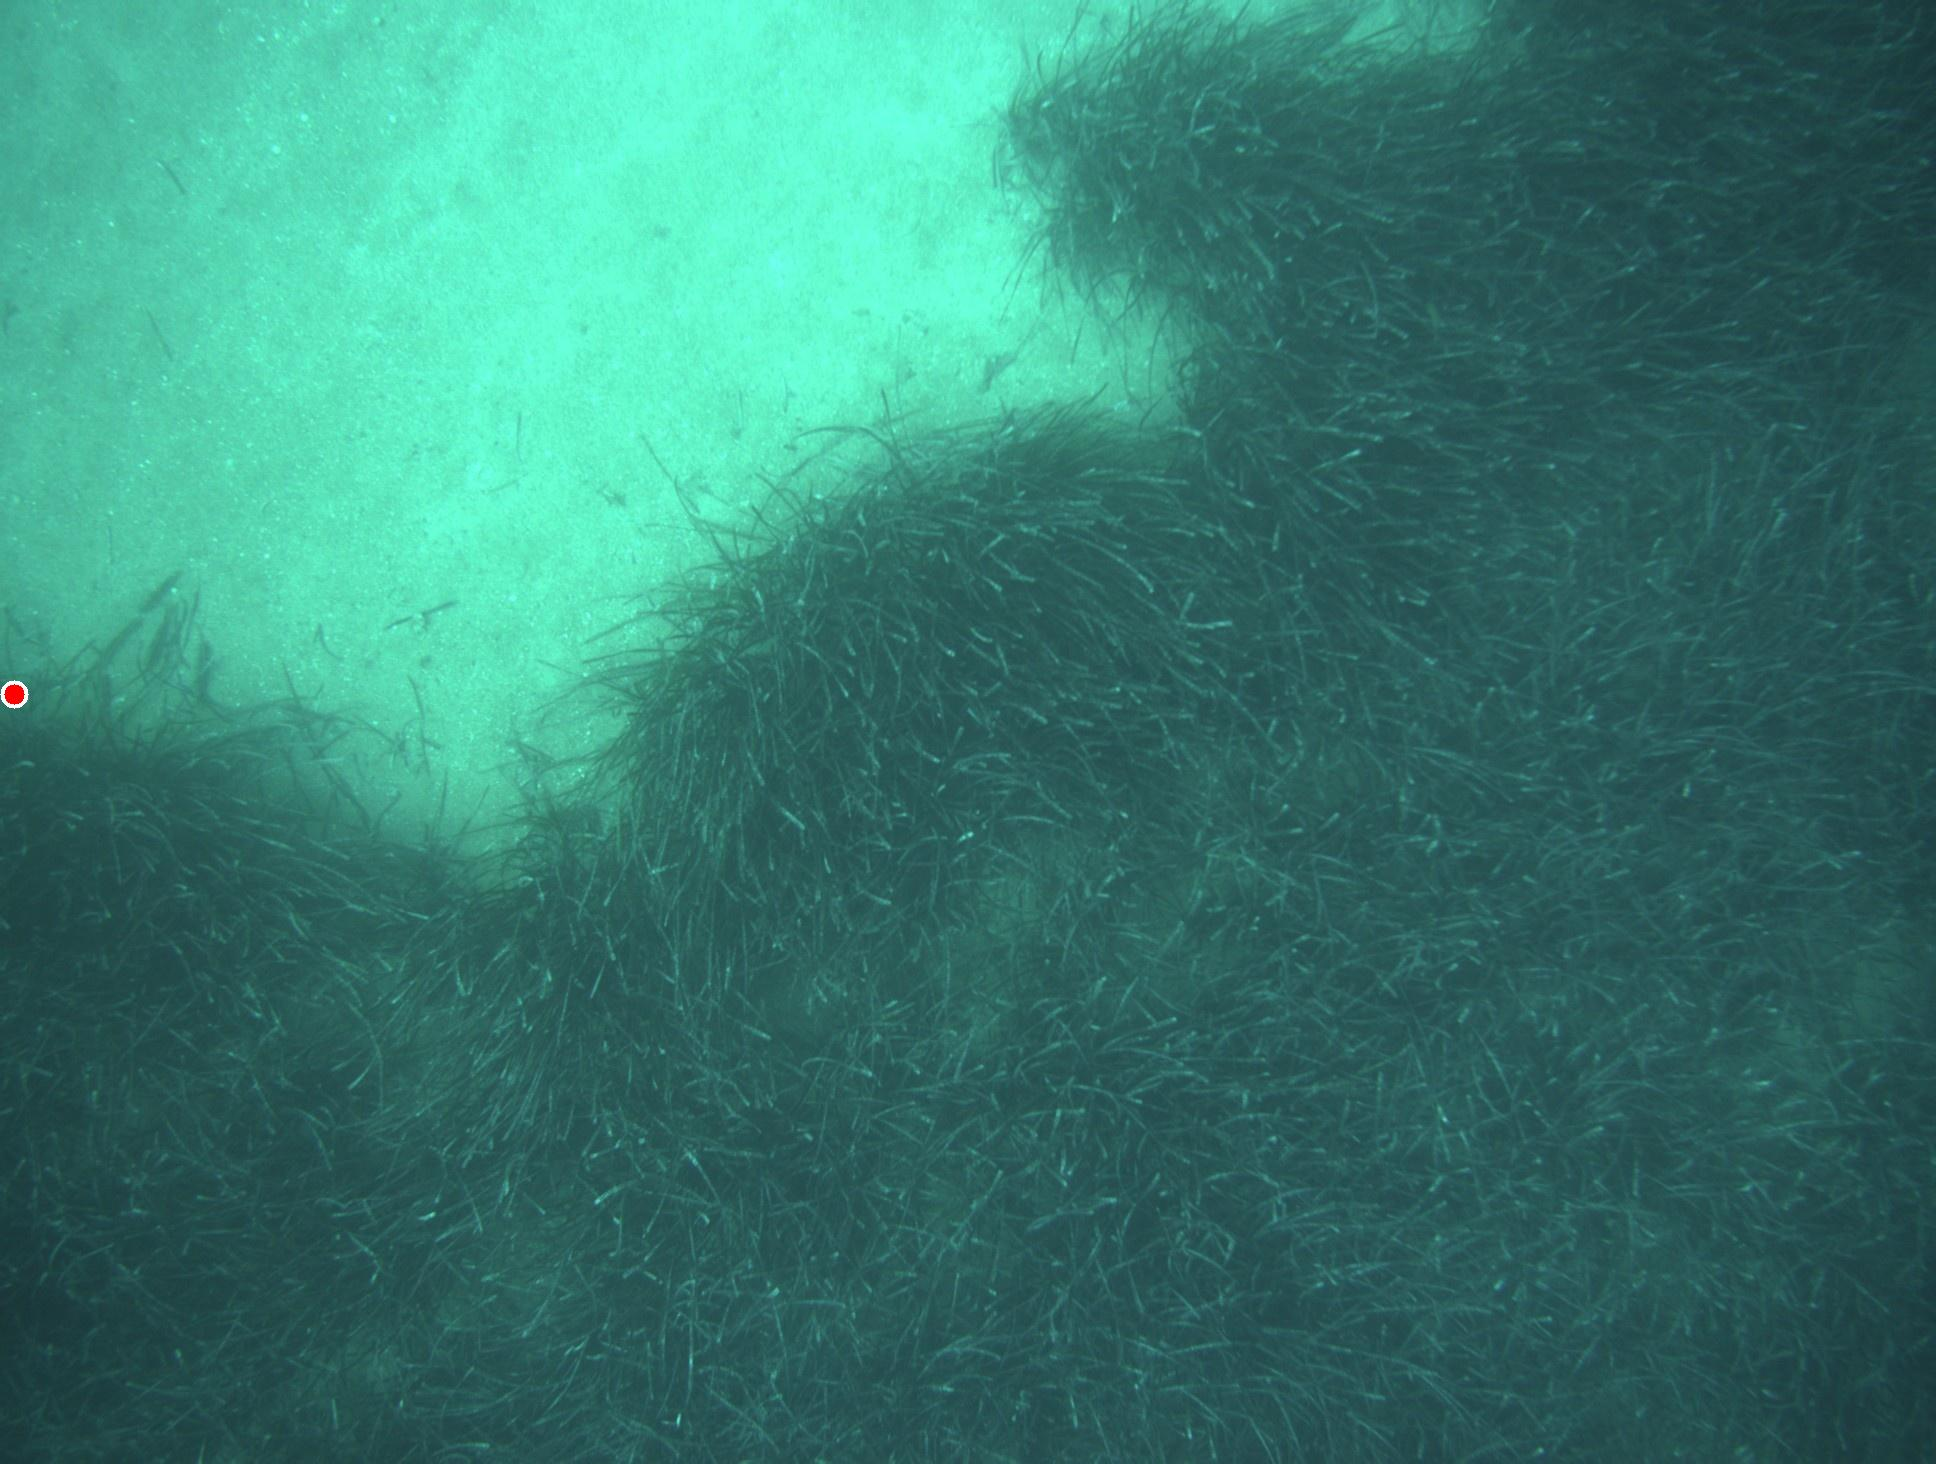
\includegraphics[width=\linewidth]{results/seagrass/registration/optical5.jpeg}
    \end{subfigure}
    &
    \begin{subfigure}[b]{0.30\linewidth}
      \centering
      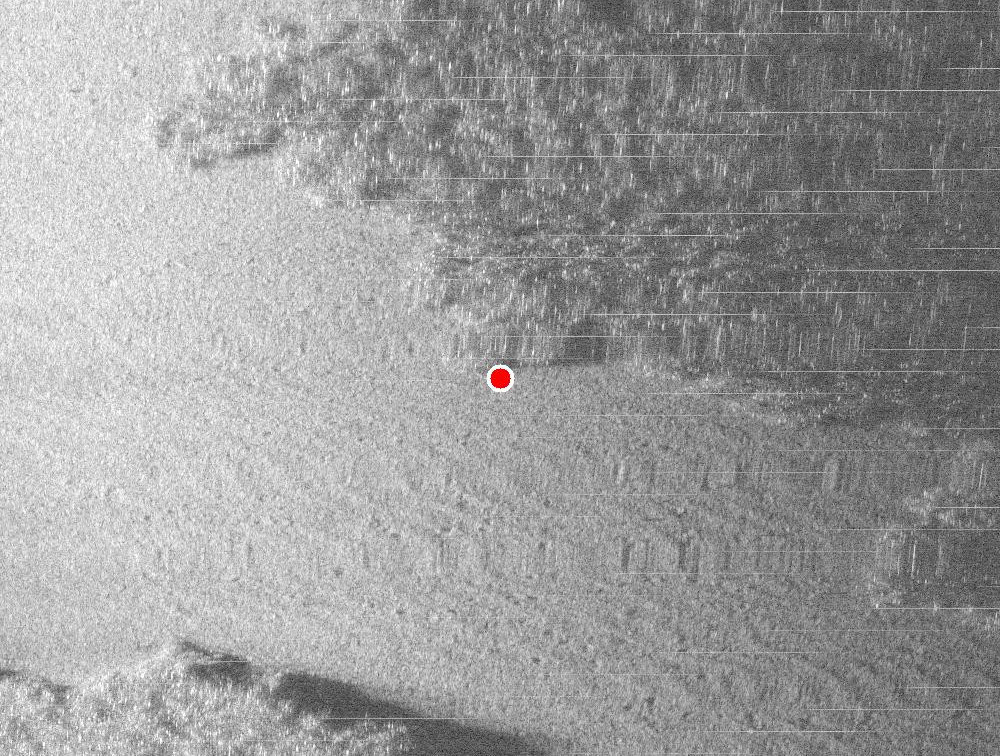
\includegraphics[width=\linewidth]{results/seagrass/registration/sss5.jpeg}
    \end{subfigure}
  \end{tabular}
  \caption{Geometric opti-acoustic co-registration results between the pointcloud (left), optical images (center), and SSS waterfall (right).}
  \label{fig:results_registration}
\end{figure}

Opti-acoustic co-registration is achieved by leveraging the geometric constraints of a Structure-from-Motion (SfM) optimization. The SfM pipeline reconstructs a sparse 3D point cloud while inherently preserving the 3D-to-2D correspondences between the synthesized 3D points and their source optical pixels. 

By spatially associating localized side-scan sonar (SSS) acoustic bins with this SfM point cloud, the geometric projection approach used for SSS waterfall alignment was extended through the following process:
\begin{itemize}
    \item \textbf{Spatial Filtering:} The spatial association radius was constrained to $1\text{~cm}$ (down from a $5\text{~cm}$ initial tolerance), isolating 3D points with near-perfect spatial intersection to the acoustic projection plane.
    \item \textbf{Pixel-Level Mapping:} Because the retained 3D points preserve their 2D optical pixel mappings, this spatial bridge establishes a deterministic, pixel-accurate co-registration between the high-resolution optical imagery and the SSS waterfall.
\end{itemize}

This deterministic alignment eliminates spatial ambiguity in multi-modal underwater sensor fusion. The resulting cross-modal dataset serves as a high-fidelity proxy for ground truth, enabling the training of Self-Supervised Learning (SSL) architectures for benthic classification and habitat mapping without requiring manual acoustic annotations.

\section{Conclusion and Future Work}

This thesis presented a novel self-supervised learning framework based on DINOv3 \cite{oriane2025} for robust, view-invariant feature matching in SSS imagery. While traditional methods like SIFT struggle with acoustic scattering, speckle noise, non-linear intensity variations, and geometric distortions \cite{lowe2004, katrusha2025}, our approach successfully mitigates these challenges. By integrating a lightweight ConvNeXt-tiny backbone \cite{liu2022, ConvNextV2}, the framework balances high feature expressiveness with the strict computational constraints inherent to AUV deployment. Furthermore, incorporating a Lambertian physics model disentangles viewpoint-dependent artifacts from intrinsic seabed reflectivity, yielding highly stable semantic representations \cite{can2025_physdnet, yvan_petillot}. Although initial qualitative results demonstrate coherent semantic feature extraction, systematic quantitative validation remains the immediate next step.

\subsection{Future Work}
Future work will focus on rigorous quantitative evaluation and framework refinement through three primary avenues:

\begin{itemize}
    \item \textbf{Ablation Studies:} Upcoming ablation studies will evaluate downstream performance via linear probing or segmentation heads across various ConvNeXt backbone stages. This will identify which layers optimize the trade-off between high-frequency sediment textures and global context \cite{oquab2024}, using unsupervised metrics like silhouette width to measure cluster tightness and separation \cite{silhoutte_ablation}.
    \item \textbf{Advanced Acoustic Modeling:} Framework fidelity can be improved by replacing the Lambertian approximation with advanced acoustic scattering models and bathymetric priors to better capture complex, heterogeneous seabeds \cite{can2025_physdnet, yvan_petillot}.
    \item \textbf{Synthetic Benchmarking:} Utilizing synthetic data generated from isolated reflectivity values will provide a rigorous benchmark to evaluate the framework's novel-view generation capabilities.
\end{itemize}


% --- SECTION 3: BIBLIOGRAPHY ---

\bibliographystyle{IEEEtran}
\bibliography{references}
\end{document}
